\documentclass[12pt,jafontscale=0.9247]{jlreq}
%\documentclass[10pt,twocolumn,column_gap=2zw]{jlreq}
%%%%%%%%%%%%%%%%%%%%%%%%%%%%
%% 欧文TTF/OTFフォントを利用するにはfontspec.styをロードする必要あり
%% 和文TTF/OTFフォントを利用するにはluatexja-fontspec.styをロードする必要あり
%% luatexja-fontspec.styはfontspec.styをないぶてきにロードする
%% lualatex-ja-preset.sty は luatexja-fontspec.styをロードする
%% つまり次の1行でluatexja-fontspec.sty, fontspec.styも自動的にロードされる
\usepackage[no-math,deluxe,expert,yu-win10]{luatexja-preset}
%%%%
\usepackage{graphicx}
\usepackage[svgnames,table]{xcolor}
\usepackage{pxrubrica}
\usepackage[default]{fontsetup}
%%%% tabular環境の改良版
\usepackage{tabularray}
\UseTblrLibrary{booktabs}
\let\textipa\relax
\usepackage{tipa}
\usepackage{enumitem}
\usepackage{multirow}
\usepackage{lmodern}
\usepackage{worldflags}
%%%%%%%%%%%%%%%%%%%%%%%%%%%%%
\usepackage{media9}
%%%%%%%%%%%%%%%%%%%%%%%%%%%%%
% Define custom pastel colors
\definecolor{customLightBlue}{RGB}{173, 216, 230}
\definecolor{customLightCyan}{RGB}{224, 255, 255}
\definecolor{customLightGreen}{RGB}{144, 238, 144}
\definecolor{customLightYellow}{RGB}{255, 255, 224}
\definecolor{customLightPink}{RGB}{255, 182, 193}
\definecolor{customLightGray}{RGB}{211, 211, 211}
\definecolor{customLavender}{RGB}{230, 230, 250}
%%%%%%%%%%%%%%%%%%%%%%%%%%%%
%% for tikzducks
\definecolor{skin}{RGB}{255,209,181}
\definecolor{lblue}{RGB}{176,172,188}
\definecolor{lbrown}{RGB}{236,213,163}
\definecolor{dbrown}{RGB}{176,134,95}
\definecolor{billcol}{RGB}{230,132,82}
%%%%%%%%%%%%%%%%%%%%%%%%%%%%%
\usepackage[at]{easylist}
%%%%%%%%%%%%%%%%%%%%%%%%%%%%
\usepackage{tikz}
\usepackage{tikzducks}
\usepackage{tikzlings,tikzsymbols}
\usetikzlibrary{arrows}
\usepackage{tcolorbox}
\newtcolorbox[auto counter, number within=section]{pabox}[2][]{%
colback=yellow!5,fonttitle=\bfseries,
title=Question~\thetcbcounter: #2,#1}
\tcbuselibrary{skins,breakable}
%%%%%%%%%%%%%%%%%%%%%%%%%%%%%
\usepackage{enumitem}%%[label=\textbf{\arabic*}]
\usepackage{ascmac}
%%%%%%%%%%%%%%%%%%%%%%%%%%%%
\usepackage{luatexja-otf}
\ltjsetparameter{jacharrange={-2}}
%%%%%%%%%%
\usepackage{longtable}
\usepackage{datetime}
% Coffeecupを一時退避(tikzsymbols版を保存)
\let\tikzCoffeecup\Coffeecup
\let\Coffeecup\relax
\let\Heart\relax
\let\Smiley\relax

\usepackage{marvosym,utfsym,circledsteps}
%\usepackage{figchild}
\usepackage{cookingsymbols}
%%%%%%%%%%%%%%%%%%%%%%%%%%%%%%
\pagestyle{empty}
%%%% ハイパーリンク
%%%% hyperref.sty は preamble の最後で読み込む
\usepackage{hyperref}
\usepackage{xurl}
\hypersetup{
  bookmarks=true,
  bookmarksnumbered=true,
  pdfauthor={iotsuka1958}
}
%%%%%%%%%%%%%%%%%%%%%%%%%%%%%
\usepackage{litetable, twemojis}
\usepackage[mono = false]{libertine}
\usepackage{ulem}
\usetikzlibrary{calendar,positioning}
%%%%%%%%%%%%%%%%%%%%%%%%%%%
%\makeatletter
%\newcommand*{\themonth}{\two@digits\month}
%\newcommand*{\theday}{\two@digits\day}
%\makeatother
%\newcommand{\mytoday}{{\the\year}年{\themonth}月{\theday}日}
\newcommand{\mytoday}{{\the\year}年{\the\month}月{\the\day}日}
%%%%%%%%%%%%%%%%%%%%%%%%%%%
\usepackage{datetime2}
\usepackage{datetime2-calc}
\makeatletter
\newcommand{\DOWjpn}{%
	\DTMcomputedayofweekindex{\@dtm@currentyear-\@dtm@currentmonth-\@dtm@currentday}{\DOWindex}%
	\ifcase\DOWindex 月\or 火\or 水\or 木\or 金\or 土\or 日\fi%
}
\newcommand{\DTMjpn}{%
	\@dtm@currentyear/\@dtm@currentmonth/\@dtm@currentday(\DOWjpn)%
}
\makeatother
%%%%%%%%%%%%%%%%%%%%%%%%%%%%%
\begin{document}
\tikzCoffeecup
\begin{tikzpicture}
 \pig
\end{tikzpicture}

\scalebox{5}{\Fork}

%\fcKettle{0.1}{black}{.5}

\scalebox{2}{\Cat}

{\gtfamily\bfseries
Goob Morning! みなさん、おはようございます。
%Hello! みなさん、こんにちは。
お元気でいらっしゃいますか

ごきげんいかがでしょう

\mytoday{}、\DOWjpn{}曜日、
時刻は
午前10時20分
%午前11時20分
%午後1時
%午後2時
をまわったところです。

きょうも、この授業は千葉市の幕張からお送りしていますが、
音声はちゃんと届いていますか。

さてきょうの幕張は、台風15号の影響を受けて、雨が激しく降っています。
昼過ぎから夜のはじめ頃にかけて雷を伴い非常に激しく降る所があるそうです。
みなさんのお住まいの地域はいかがでしょうか。
%千葉県には熱中症警戒アラートが発表されています。
%引き続き熱中症には十分注意してください。
%気象庁では最高気温が35度以上の日、いいですか「35度を超える」ではありません、35度以上の日を\kenten{猛暑日}と定義していますから、
%きょうは猛暑日の一歩手前まできたということですね。
%きょうも千葉県に熱中症警戒アラートが発表されています。
%幕張地区、厳しい暑さになっています。
%低い雲が垂れ込めて薄暗くなっています。
%朝から気温が高くなっています。
%幕張地区、現在、摂氏30度を超えています。
%熱中症警戒アラートも発表されています。
%強い雨になっている地域もあるようです。
%気温は30度近くまで上がっています。
%湿度も80\%を超えています。
%暑さに体が慣れない今の時期は、暑さがこたえますね。
%みなさんのお住まいの地域はいかがでしょうか。
%きょうは気圧も低くなっているので、頭が痛いなとか調子がいまひとつという人もいるかもしれませんね。
%梅雨の中休みというよりは、もう真夏のような天候が続いています。
%33度まで上昇しています。
%湿度も高くなっています。
%じめじめ、ムシムシとした不快な暑さになっています。
%じとーっと身体にこたえる感じです。
%熱中症に注意してください。
%千葉県には熱中症警戒アラートこそ発表されていないようですが、

気温は30度には徹しないようですが、
湿度は90\%を超えています。
気圧も低めのようですから、調子が出ないという人もいるでしょう。
%引き続き熱中症にはじゅうぶん警戒してください。
%適切にエアコンを利用するとともに、%
%喉が渇いたなとおもうまえに、こまめに水分補給を心がけてください。
%あわせて塩分補給もたいせつです。
%%%%%授業中も、
%手元に飲み物を用意して参加してください。

%とはいえ、どうか水分補給をお忘れなく。
%授業中だからと遠慮する必要はありません。

%きょうは\DOWjpn{}曜日。
%それでは、きょうの授業、気を楽にしてはじめていきましょう。
%今週が終われば夏休みというところまでこぎつけました。
%今週もはじまったばかりで、先が長い感じがします。
%おまけにこの暑さです。
%やっと、なんとか週のまんなかまでこぎつけた感じです。
%今週もきょうと明日の2日となりました。あともう一息というところです。
%きょうで今週も終わりです。
%みなさんもこれが今週最後の時間ですね。
%やる気があまり出ないという人もいるかとおもいますが、この授業を聞いているみなさんは、いまこの時間に参加しているだけでじゅうぶんです。
%この気候ですから、
あまり無理をしないで、
ご自身のペースで参加してください。
気負わず、肩の力を抜いて、
リラックスしておつきあいください
%
それではきょうの
授業、今週最後の英語の授業スタートしましょう
}

\newpage
%%%%%%%%%%%%%%%%%%%
\section*{Google NotebookLMで日本語字幕入り動画を作成}


google notebook lmで、
Video Overviewの機能を用いて
たとえばhoge.mp4を作成する。


\verb|create_srt.py hoge.mp4|とすると、\verb|hoge.srt|ができる。

次のコマンドで事務く入りmp4である\verb|hoge_subtitle.mp4|ができる。

\begin{verbatim}
ffmpeg -i hoge.mp4 -vf ”subtitles=hoge.srt:charenc=UTF-8” -c:v libx264 -crf 18 -preset slow -c:a copy hoge_subtitle.mp4
\end{verbatim}
もとのhoge.srtが英語の場合は、Geminiで次のようにすれば日本語のsrtファイルができる。
\begin{tcolorbox}
 以下は英語の字幕を格納したsrtファイルです。引用符でくくられた個所のみを、英語から日本語に直したsrtファイルにしてください。厳密な和訳でなく、内容を大づかみにつかんだうえで要点を抽出するようにお願いします。文章が割れているところもあるので、じっくり考えて正しく自然な日本語になるようじゅうぶん注意してください
---以下に英語のsrtをはりつける
\end{tcolorbox}

結果が出力されるので、それをコピー・アンド・ペーストして、
たとえばhoge\_ja.srtというファイル名にして次のコマンド打てば日本語字幕入りmp4が完成

\begin{verbatim}
ffmpeg -i 021_when.mp4 -vf ”subtitles=021_when_ja.srt:charenc=UTF-8” -c:v libx264 -crf 18 -preset slow -c:a copy 021_when_ja_subtitle.mp4
\end{verbatim}

%%%%%%%%%%%%%%%%%%%%
\newpage
\vfill

{\gtfamily\bfseries

みなさん、
1年生は47回、2・3年生は52回、授業がありました。
おつかれさまでした。
楽しい夏休みをお過ごしください
}

%\vfill
%
%みなさん、こんにちは。
%今日の国語の授業では、漢字の学習を行います。
%この部屋からは退出せず、画面に表示された指示に従って進めてください。
%使用するプリントや確認問題の該当番号は、国語のクラスのストリームに書いてあります。
%今日は「漢字練習プリント2の2」と「確認問題2の2」を使用します。
%では、始めてください

%\end{document}

%%%%%%%%%%%%%%%%%%%%%%%%%%
2次方程式
\[
 ax^2+bx+c=0\,\,\,\,\,\,\,\,\text(a\neq{}0\text)
\]
の解を$\alpha$, $\beta$とするとき、次の関係が成立することを示してください。

\begin{tcolorbox}
 \[
 \alpha + \beta = -\frac{b}{a}\,\,,\,\,\,\,\,\,\,\,\alpha\beta = \frac{c}{a}
\]

\end{tcolorbox}
\end{document}

\newpage
%%%%%%%%%%%%%%%%%%%%%%%%%%%
2次方程式
\[
 ax^2+bx+c=0\,\,\,\,\,\,\,\,\text(a\neq{}0\text)
\]
の解は
\[
x=\frac{-b\pm{}\sqrt{b^2-4ac}}{2a}
\]
となることを導出してみましょう。

\end{document}


%%%%%%%%%%%%%%%%%%%%%%%%%%%
\noindent{\Large\gtfamily 「エデュオプちば」懸案事項}

\hfill{}令和7年8月●日 児童生徒安全課


\subsection*{1\,\,\,\,\,学校種を越えた下学年のオンライン授業及びオンデマンド配信受講について}
 1学期末に実施した「エデュオちば」アンケート結果等を踏まえ、児童生徒安全課では学校種を越えた下学年のオンライン授業及びオンデマンド配信受講(※中学生が小学生の配信を受講)について、2学期から認めることを検討しています。ついては、皆様の御意見をお聞かせください。

\subsubsection*{(参考)中学生の1学期アンケート結果}

\begin{quote}
 \noindent{}8\,\,\,\,他の学年のオンライン授業(ライブ配信)を受けたい\\
 小6:\,\,11名(12\%)、\,\,\,\,小5:\,\,8名(8.7\%)、小4:\,\,6名(6.5\%) $\longrightarrow$計25名(27.2\%)

\smallskip

\noindent{}9\,\,\,\,他の学年のオンデマンド配信を見たい\\
 小6:\,\,14名(14.9\%)、小5:\,\,9名(9.6\%)、小4:\,\,7名(7.4\%) $\longrightarrow$ 計30名(31.9\%)
\end{quote}

\begin{tcolorbox}[title=意見]
\begin{itemize}
 \item 一般論でいえば、実現すべき
 \item いっぽうで、想定しうる課題への対応はしっかりクリアする必要がある
       \begin{itemize}
	\item 授業に上の学年の生徒が参加し、不規則な発言等があったとき、授業が混乱しないか
	\item 小中で授業時間が異なることによる問題はないか
	\item 時間割を、臨時的な授業変更も含め、上の学年にも遺漏なく周知す必要ことが必要
	\item 当日の授業で扱う分野について、どの段階でどこまで詳細に案内すべきか
	\item 授業への参加に関するログは問題なく取得・提供ができるか
	\item 現状より事務量が増加することへの対応は可能か
       \end{itemize}
\end{itemize}
\end{tcolorbox}

\newpage

\subsection*{2\,\,\,\,\,\,\,\<「エデュオプサポーター」(会計年度任用職員)の配置について}
 本年度は、授業中における児童生徒からの質問に対応するための「エデュオプサポーター」(会計年
度任用職員)の配置が予算化されています。以下の2点について、皆様の御意見をお聞かせください。

\begin{itemize}
 \item[(1)] エデュオプサポーターの必要性について
 \item[(2)] エデュオプサポーターを配置する教科及び活用方法について
\end{itemize}

\begin{tcolorbox}[title=「エデュオプサポーター」の配置についての意見]
\begin{itemize}
 \item 一般論でいえば、人が配置されることは有効と思料される。予算がついたから、配置されたからということが先行するのではなく、有効な活用方法を見出すべき
 \item この配置が既存職員の負担増となってはならない
 \item どの教科において効果的ということはない
 \item どの発達段階(小学校・中学校)において効果的ということはない
 \item 配信授業と同時にエデュオプサポーター(以下「サポーター」という。)が質問に対応する形式はきわめて困難
        \begin{itemize}
	 \item ある生徒への質問に対応している際に、サポーターとのやりとりが他の生徒の目に触れることとなり、他の生徒の集中力を妨げることとなる
	 \item サポーターに生徒が質問している間に授業が進行し、質問した生徒が授業についていけなくなる
	 \item いっぽうで、質問に対応している際に授業を止めることは、他の生徒のへの迷惑となることから、すべきではない
        \end{itemize}

\end{itemize}


以上のことから、次のような活用をお願いすることとしてはどうか

\begin{itemize}
 \item 毎時、配信授業に続く10分を、同室において主に当該授業内容に係る質問にサポーターが対応する
         \begin{itemize}
	  \item 授業に連続して質問対応の時間を設けることにより、学習内容が頭に残っているうちに生徒が質問できることとなり、学習内容の着実な理解定着に資する
	  \item サポーターが授業の内容をじゅうぶん理解した上で、合理的かつ効果的な説明が可能になる
	  \item 授業時にそのつど質問を受け対応することにより生じる他の生徒へのマイナスの影響を避けることができる
	 \end{itemize}
 \item その他、以下のようなこともお願いできればいいのではないか
          \begin{itemize}
         \item 教科や単元によるが、配信授業の中で一定時間を演習に充当し、その時間内に別室でサポーターが質問に対応する。その間、授業は中断し作業の時間とする。(ただし、この手法であっても、毎時間一定時間の演習を設けることは難しい。)
	   \item 授業を展開する上で、必要な補助。例えば一人では難しい実験の補助など
	   \item オンデマンドの動画がよりわかりやすいものになるよう、動画の画像編集・音声調整及びアップロード作業
	  \end{itemize}
\end{itemize}
\end{tcolorbox}
%%%%%%%%%%%%%%%%%%%%%%%%%%%%
\subsection*{メディア棟1階児童生徒安全課執務室(エデュオプちば)}
\large

いつもお世話になります

生ごみの回収は、いったん休止し、9月からふたたびお願いします

\worldflag[width=2cm,framewidth=0.3mm,framecolor=black]{BR}
%%%%%%%%%%%%%%%%%%%%%%%%%%
\newpage
\subsection*{メディア棟1階児童生徒安全課執務室(エデュオプちば)}
いつもお世話になります

紙の回収は、いったん休止し、9月からふたたびお願いします

\normalsize
%%%%%%%%%%%%%%%%%%%%%%%%%%%
\newpage
%%%%%%%%%%%%%%%%%%%%%%%%%%
%\includemedia[
%width=0.6\linewidth,height=0.3375\linewidth, % 16:9
%activate=pageopen,
%flashvars={
%modestbranding=1 % no YT logo in control bar
%&autohide=1 % controlbar autohide
%&showinfo=0 % no title and other info before start
%&rel=0 % no related videos after end
%}
%]{}{http://www.youtube.com/v/r382kfkqAF4?rel=0}


%%%%%%%%%%%%%%%%%%%%%%
\newpage
\tikz \calendar[dates=2025-01-01 to 2025-12-last,week list,
                month label above centered];
%%%%%%%%%%%%%%%%%%%%%%%
\newpage
\tikz[baseline=0pt]
  \calendar
    [dates=2025-01-01 to 2025-01-last,week list,
     month label above centered,
    month text=\%mt \%y0]
    if (Sunday) [red]
    if (Saturday) [blue]
    if (between=2025-01-01 and 2025-01-03) [red]
    if (equals=2025-01-13) [red];
\hspace{10pt}
\tikz[baseline=0pt]
  \calendar
    [dates=2025-02-01 to 2025-02-last,week list,
     month label above centered,
    month text=\%mt \%y0]
    if (Sunday) [red]
    if (Saturday) [blue]
    if (equals=2025-02-11) [red]
    if (equals=2025-02-24) [red];
\hspace{10pt}
\tikz[baseline=0pt]
  \calendar
    [dates=2025-03-01 to 2025-03-last,week list,
     month label above centered,
    month text=\%mt \%y0]
    if (Sunday) [red]
    if (Saturday) [blue]
    if (equals=2025-03-20) [red];
%%%%%%%%%%%%%

\bigskip

\tikz[baseline=0pt]
  \calendar
    [dates=2025-04-01 to 2025-04-last,week list,
     month label above centered,
    month text=\%mt \%y0]
    if (Sunday) [red]
    if (Saturday) [blue]
    if (equals=2025-04-29) [red];
\hspace{10pt}
\tikz[baseline=0pt]
  \calendar
    [dates=2025-05-01 to 2025-05-last,week list,
     month label above centered,
    month text=\%mt \%y0]
    if (Sunday) [red]
    if (Saturday) [blue]
    if (between=2025-05-03 and 2025-05-06) [red]
    if (equals=2025-02-24) [red];
\hspace{10pt}
\tikz[baseline=0pt]
  \calendar
    [dates=2025-06-01 to 2025-06-last,week list,
     month label above centered,
    month text=\%mt \%y0]
    if (Sunday) [red]
    if (Saturday) [blue];
%%%%%%%%%%%%%

\bigskip

\tikz[baseline=0pt]
  \calendar
    [dates=2025-07-01 to 2025-07-last,week list,
     month label above centered,
    month text=\%mt \%y0]
    if (Sunday) [red]
    if (Saturday) [blue]
    if (equals=2025-07-21) [red];
\hspace{10pt}
\tikz[baseline=0pt]
  \calendar
    [dates=2025-08-01 to 2025-08-last,week list,
     month label above centered,
    month text=\%mt \%y0]
    if (between=2025-08-18 and 2025-08-29) [yellow]
    if (Sunday) [red]
    if (Saturday) [blue]
    if (equals=2025-08-11) [red];
\hspace{10pt}
\tikz[baseline=0pt]
  \calendar
    [dates=2025-09-01 to 2025-09-last,week list,
     month label above centered,
    month text=\%mt \%y0]
    if (Sunday) [red]
    if (Saturday) [blue]
    if (equals=2025-09-15) [red]
    if (equals=2025-09-23) [red];
%%%%%%%%%%%%%

\bigskip

\tikz[baseline=0pt]
  \calendar
    [dates=2025-010-01 to 2025-10-last,week list,
     month label above centered,
    month text=\%mt \%y0]
    if (Sunday) [red]
    if (Saturday) [blue]
    if (equals=2025-10-13) [red];
\hspace{10pt}
\tikz[baseline=0pt]
  \calendar
    [dates=2025-11-01 to 2025-11-last,week list,
     month label above centered,
    month text=\%mt \%y0]
    if (Sunday) [red]
    if (Saturday) [blue]
    if (equals=2025-11-03) [red]
    if (equals=2025-11-24) [red]
    if (between=2025-11-04 and 2025-11-07) [yellow];
\hspace{10pt}
\tikz[baseline=0pt]
  \calendar
    [dates=2025-12-01 to 2025-12-last,week list,
     month label above centered,
    month text=\%mt \%y0]
    if (Sunday) [red]
    if (Saturday) [blue]
    if (between=2025-12-29 and 2025-12-last) [red];
%%%%%%%%%%%%%%

\bigskip

\tikz[baseline=0pt]
  \calendar
    [dates=2026-01-01 to 2026-01-last,week list,
     month label above centered,
    month text=\%mt \%y0]
    if (Sunday) [red]
    if (Saturday) [blue]
    if (between=2026-01-01 and 2026-01-03) [red]
    if (equals=2025-01-12) [red];
\hspace{10pt}
\tikz[baseline=0pt]
  \calendar
    [dates=2026-02-01 to 2026-02-last,week list,
     month label above centered,
    month text=\%mt \%y0]
    if (Sunday) [red]
    if (Saturday) [blue]
    if (equals=2026-02-11) [red]
    if (equals=2026-02-23) [red];
\hspace{10pt}
\tikz[baseline=0pt]
  \calendar
    [dates=2026-03-01 to 2026-03-last,week list,
     month label above centered,
    month text=\%mt \%y0]
    if (Sunday) [red]
    if (Saturday) [blue]
    if (equals=2026-03-20) [red];
%%%%%%%%%%%%%%%%%%%%%%%%%%
\newpage
\begin{itemize}
 \item オンライン授業の経験もない
 \item 中学生を相手にするのもはじめて
 \item そもそも授業自体が30年ぶりくらい
\end{itemize}

いってみれば三重苦というか、まったくベースがない状態でのスタート

テクニカルな事項についてはずぶの素人であり、
とにかく手取り足取りで教えていただいた、というか全面的に支えていただきました

授業の中身については、これは教える側の基礎的な学力といいいますかそもそもの素養や教養が問われるところであるが、
急にどうにかなるものではないので、一種の開き直り

授業のスタイル的には、まわりのみなさんはいろいろと創意工夫をしながら展開したものと
承知しているが、
自分はスライド、あ、これただのpdfですが、これでたんたんと進めた。まあいってみれば芸がない感じかとおもうのですが、
長丁場であり自分で持続できるやり方でやるしかないかなと。
ということでホワイトボードとか書画カメラは使用しなかった。
こちらについては数学の佐藤啓之さんから詳しいガイダンスがあるでしょう。
スライドはただのpdfファイル

\begin{itemize}
 \item 前時に参加していると限らないことから、前時の内容を当然のこととして進めるのではなく、ある程度さかのぼった説明をする
 \item 前時に参加していた生徒にとってはまだるっこしい部分が出てくる。また進度に影響が
 \item 40分授業ということで、生徒の集中力が途切れがちの印象。発達段階や不登校であることを考慮したとき、40分という時間が妥当なのか疑問
 \item 区切りがあるので、毎回40分と機械的に固定するのがいいとはおもえない
 \item 授業の焦点をどこにあわせればいいのか。生徒の学力レベルの把握が困難
 \item インタラクティブを意識し、クイズやゲーム形式、かんたんな作業を取り入れるようしている
 \item 双方向性を意識し、チャットでの回答やリアクションスタンプを活用しているが、反応するのは特定の生徒に偏る印象
 \item 予習はしなくていいといっている。復習は可能ならしましょう。宿題はださない
 \item 教材、スライドの準備がきわめて煩瑣・事務量がはんぱではない(通常の教室での授業、対面での授業の比ではない)しかも週12コマすべて異なる内容のスライドの準備
\end{itemize}


%%%%%%%%%%%%%%%%%%%%%%%%%%
\newpage
\thispagestyle{empty}

\noindent{}様式1\hfill\mbox{}


\mbox{}\hfill{\bfseries 公務に使用する自家用自動車等登録・取消申請書}\hfill\mbox{}

\mbox{}\hfill{}令和7年4月1日

\bigskip

千葉県立千葉中学校長 様

\bigskip

\mbox{}\hfill\begin{tabular}{ll}
	      職&臨時的任用講師 \\
              指名&大塚一朗 \\
	     \end{tabular}

\bigskip

公務に使用する自家用自動車等の登録について、
職員の自家用自動車等の公務使用に関する取扱要綱第5条第1項の規定により、
下記のとおり申請します。

\mbox{}\hfill{}記\hfill\mbox{}

\bigskip

\begin{tabular}{|l|l|l|}\hline
 \multicolumn{2}{|l|}{登録・取消の別} & 登録     \sout{取消}\\\hline
 \multicolumn{2}{|l|}{申請者の免許取得年月日   } & \\\hline
 \multicolumn{2}{|l|}{申請者の免許有効期限} & 令和7年7月19日\\\hline
 \multicolumn{2}{|l|}{車種・車両番号} & \\\hline
 \multicolumn{2}{|l|}{型式・排気量} & \\\hline
 \multicolumn{2}{|l|}{所有者氏名} & 本人\\\hline
 \multicolumn{2}{|l|}{自動車検査証有効期間} & \\\hline
 \multicolumn{2}{|l|}{自賠責保険有効期間} & \\\hline
 \multirow{4}{1.1\zw}{任\\[-4pt]意\\[-4pt]保\\[-4pt]険\\[-4pt]等}& 
\multirow{2}{*}{加入内容}& 対人 無制限       対物 1,000万円    \\\cline{3-3}
 & & その他\\\cline{2-3}
 & 有効期間& 令和7年11月27日\\\cline{2-3}
 & 保険会社名& \\\hline
 \multicolumn{2}{|l|}{乗用車ヘルメットの所持} & 有・無\\\hline

\end{tabular}

\bigskip

備考
\begin{enumerate}
 \item この申請書には、申請者の運転免許証、自動車検査証、自賠責保険証明所及び
任意保険の証書等、記載内容を証する書類の各写しを添付すること
 \item 登録の対象が250cc以下の自動二輪車又は原動機付自転車の場合は、自動車検査証有効期間の欄は記載不要であること
 \item 登録の対象が自転車の場合は、車種・車両番号の欄に「自転車」と記載の上、
任意保険等の欄に自転車損害賠償保険等の内容を、乗車用ヘルメットの所持の欄に所持の有無を記載すること
 \item 取消の場合は、車種・車両番号の欄のみを記載すること
\end{enumerate}
%%%%%%%%%%%%%%%%%%%%%%%%%%%%%%%%%
\iffalse
\begin{enumerate}\setcounter{enumi}{1}
 \item $\left\{\begin{tabular}{rl}
		(A)& I \textcolor{Maroon}{\bfseries watched} the movie two years ago.\hspace{9\zw}{\scriptsize movie \textipa{/m\'u:vi/} 映画}\\
(B)& I \textcolor{NavyBlue}{\bfseries have watched} the movie three times.
\end{tabular}
\right.$
\end{enumerate}
\fi
%%%%%%%%%%%%%%%%%%%%%%%%%
\newpage

\# 命令書:
あなたは、アメリカ人のプロの英語講師です。
以下の制約条件をもとに、英語の読み物教材を作成してください

\# 制約条件:
・想定する読者は英語初級者である
・平易な英文でまとめること
・中学生が興味をもつトピック
・分量は100語程度
・would like toという表現を含むこと
・読後の生徒の理解度を試す正誤問題を5問付すこと
%%%%%%%%%%%%%%%%%%%%%%%%%%%%%%%%%%%%%%%
\newpage
\weeklist [ format = \bfseries \scshape, sep = \textbar ]
{
\texttwemoji{1f312} Mon -> 1, \texttwemoji{1f525} Tue -> 1,
\texttwemoji{1f30a} Wed -> 1, \texttwemoji{1f332} Thu -> 1,
\texttwemoji{1fa99} Fri -> 1
}
\timelist [ numformat = \ttfamily \bfseries, timeformat = \ttfamily ]
{
08:05 -> 08:50, 08:55 -> 09:40, 10:20 -> 11:00, 11:00 -> 11:20,
11:20 -> 12:00, 12:00 -> 13:00, 13:00 -> 13:40, 13:40 -> 14:00,
14:00 -> 14:40, 18:30 -> 19:15, 19:20 -> 20:05, 20:10 -> 20:55
}
\begin{litetable} [ MidnightBlue, sem = SEM 1 ] { Course Schedule }
\newday
\course [ subject = interface3, comment = \TeX{} Live 2025,
lecture = The \LaTeX{} Project, DarkBlue ] {4} {5}
\newday
\course [ subject = expl3, lecture = The \LaTeX{} Project ] {8} {8}
\newday
\course [ subject = Keep on \TeX ing, lecture = Donald E. Knuth,
location = Stanford University, Purple ] {10} {11}
\newday
\course [ subject = Ti\textit k\/Z, lecture = \textsc{pgf},
Crimson, comment = Version 3.1.10 ] {3} {5}
\more { Programme Duration: 09 / 2021 -- 07 / 2025 }
\end{litetable}

%%%%%%%%%%%%%%%%%%%%%%%%%%
\newpage
\begin{center}
 English Slides
\end{center}

\scriptsize
\begin{longtblr}[caption={English Slides}]{
  width = { 0.95\linewidth },
  colspec= {lll},
%  row{2-5,8-12,15,36-37,40} = {bg = yellow!50},
  rowhead=1,
  hline{1,Z} = { 0.08em }, % 表の最上と最下に太さ 0.08em の横罫線
  hline{2} = { 0.05em } % 表の1行目の下の横罫線
}
path & file\_name & mp3 \\ 
./orientation/ & orientation.tex & - \\ 
./orientation/ & orientation\_2.tex & - \\ 
./1st\_grader/ & 999quiz.tex & TRUE \\ 
./1st\_grader/ & 999quiz\_full\_vesion.tex & TRUE \\ 
./1st\_grader/ & 099\_pronunciation.tex & TRUE \\ 
./pronunciation/ & pronunciation\_consonant.tex & TRUE \\ 
./pronunciation/ & pronunciation\_vowel.tex & TRUE \\ 
./pronunciation/ & pronunciation\_japanese.tex & TRUE \\ 
./1st\_grader/ & 001\_alphabet.tex & TRUE \\ 
./1st\_grader/ & 002\_sv.tex & TRUE \\ 
./1st\_grader/ & 003\_be.tex & TRUE \\ 
./1st\_grader/ & 004\_verb.tex & TRUE \\ 
./1st\_grader/ & 004\_verb\_object.tex & TRUE \\ 
./1st\_grader/ & 005\_pronoun.tex & TRUE \\ 
./1st\_grader/ & 005\_singular\_plural.tex & TRUE \\ 
./1st\_grader/ & 006\_negative\_be.tex & TRUE \\ 
./1st\_grader/ & 007\_negative\_do.tex & TRUE \\ 
./1st\_grader/ & 008\_question\_be.tex & TRUE \\ 
./1st\_grader/ & 009\_answer\_be.tex & TRUE \\ 
./1st\_grader/ & 010\_question\_do.tex & TRUE \\ 
./1st\_grader/ & 011\_answer\_do.tex & TRUE \\ 
./1st\_grader/ & 012\_can.tex & TRUE \\ 
./1st\_grader/ & 013\_who.tex & TRUE \\ 
./1st\_grader/ & 014\_when.tex & TRUE \\ 
./1st\_grader/ & 015\_where.tex & TRUE \\ 
./1st\_grader/ & 016\_which.tex & TRUE \\ 
./1st\_grader/ & 017\_how.tex & TRUE \\ 
./1st\_grader/ & 018\_why.tex & TRUE \\ 
./1st\_grader/ & 019\_what.tex & TRUE \\ 
./1st\_grader/ & 020\_whose.tex & TRUE \\ 
./1st\_grader/ & 020a\_who.tex & TRUE \\ 
./1st\_grader/ & 021\_is\_ing\_intro.tex & TRUE \\ 
./1st\_grader/ & 022\_is\_ing\_negative.tex & TRUE \\ 
./1st\_grader/ & 023\_is\_ing\_question.tex & TRUE \\ 
./1st\_grader/ & 024\_past\_be.tex & TRUE \\ 
./1st\_grader/ & 025\_past\_do.tex & TRUE \\ 
./1st\_grader/ & 026\_past\_didnot.tex & TRUE \\ 
./1st\_grader/ & 027\_past\_did\_you.tex & TRUE \\ 
./1st\_grader/ & 032\_imperative.tex & TRUE \\ 
./1st\_grader/ & 033\_exclamatory.tex & TRUE \\ 
./2nd\_grader/ & 001\_there\_is.tex & TRUE \\ 
./2nd\_grader/ & 005\_was\_ing\_intro.tex & TRUE \\ 
./2nd\_grader/ & 011\_be\_going\_to.tex & TRUE \\ 
./2nd\_grader/ & 012\_will.tex & TRUE \\ 
./2nd\_grader/ & 013\_must.tex & TRUE \\ 
./2nd\_grader/ & 014\_have\_to.tex & TRUE \\ 
./2nd\_grader/ & 020\_part\_of\_speech.tex & TRUE \\ 
./2nd\_grader/ & 021\_when.tex & TRUE \\ 
./2nd\_grader/ & 022\_if.tex & TRUE \\ 
./2nd\_grader/ & 023\_because.tex & TRUE \\ 
./2nd\_grader/ & 031\_infinitive\_intro.tex & TRUE \\ 
./2nd\_grader/ & 032\_infinitive\_noun.tex & TRUE \\ 
./2nd\_grader/ & 033\_infinitive\_adj.tex & TRUE \\ 
./2nd\_grader/ & 034\_infinitive\_adv.tex & TRUE \\ 
./2nd\_grader/ & 035\_wh\_to\_do.tex & TRUE \\ 
./2nd\_grader/ & 036\_gerund.tex & TRUE \\ 
./2nd\_grader/ & 041\_as\_as.tex & TRUE \\ 
./2nd\_grader/ & 042\_er.tex & TRUE \\ 
./2nd\_grader/ & 043\_est.tex & TRUE \\ 
./2nd\_grader/ & 044\_more\_most.tex & TRUE \\ 
./2nd\_grader/ & 045\_better\_best.tex & TRUE \\ 
./2nd\_grader/ & 051\_passive.tex & TRUE \\ 
./3rd\_grader/ & 011\_have\_pp\_intro.tex & TRUE \\ 
./3rd\_grader/ & 012\_have\_pp\_keizoku.tex & TRUE \\ 
./3rd\_grader/ & 013\_have\_pp\_keiken.tex & TRUE \\ 
./3rd\_grader/ & 014\_have\_pp\_kekka.tex & TRUE \\ 
./3rd\_grader/ & 021\_N\_ing.tex & TRUE \\ 
./3rd\_grader/ & 022\_N\_pp.tex & TRUE \\ 
./3rd\_grader/ & 031\_N\_wh\_V.tex & - \\ 
./3rd\_grader/ & 032\_N\_wh\_SV.tex & - \\ 
./3rd\_grader/ & 041\_mood\_intro.tex & TRUE \\ 
./3rd\_grader/ & 042\_mood\_i\_wish.tex & TRUE \\ 
./3rd\_grader/ & 043\_mood\_if.tex & TRUE \\ 
\end{longtblr}

\normalsize


%%%%%%%%%%%%%%%%%%%%%%%%
\newpage
hoge
\begin{tikzpicture}

  \fill[black] (-0.1,0.4) rectangle (1.9,2.8);

  \clip (-0.1,0.4) rectangle (1.9,2.8);


  \duck[
    body=skin,
    jacket=dbrown!10!white,
    bill=billcol
  ]
  
   \fill[dbrown]  (0.490,1.145) .. controls (0.267, 1.102) and (-0.125,0.657) .. (0.289,0.261) .. controls (0.704,-0.135) and ( 2.863,0.130) .. (1.818,1.419) .. controls (0.880, 0.946) and ( 1.240,1.378) .. (0.46,0.55) -- cycle;
  
  \begin{scope}[scale=0.12,xshift=-1.3cm,yshift=3.8cm]
    \fill[lbrown] (7.7941,13.7509) .. controls (10.8320,13.4186) and (11.7764,12.3930) .. (12.6964,10.9465) .. controls (12.6964,10.9465) and (12.6769,5.6002) .. (12.9122,2.0156) .. controls (13.2041,1.7780) and (13.7523,1.8952) .. (14.0339,2.1451) .. controls (14.2660,2.3512) and (13.9970,2.8707) .. (14.2496,3.0512) .. controls (14.6140,3.3115) and (15.1783,2.7387) .. (15.5871,2.9217) .. controls (15.8312,3.0309) and (16.0169,3.3052) .. (16.0616,3.5688) .. controls (16.0616,3.5688) and (14.7664,8.8740) .. (13.1278,13.5783) .. controls (11.9515,15.3829) and (8.6715,16.0161) .. (7.7941,13.7509) -- cycle;
    \fill[lblue] (4.9884,10.6533) .. controls (7.4488,14.0291) and (12.6964,7.7969) .. (12.6964,7.7969) .. controls (13.4861,7.8582) and (13.1708,10.7423) .. (12.8259,11.2053) .. controls (10.9927,13.8335) and (9.2448,13.7940) .. (9.2448,13.7940) .. controls (6.4433,14.0475) and (4.8380,11.8428) .. (4.9884,10.6533) -- cycle;
  \end{scope}
  
  \fill[gray!80!white] (1.24,1.35) circle[radius=0.06];
  \fill[white] (1.225,1.365) ellipse[x radius=0.015, y radius=0.03,rotate=-30];
\end{tikzpicture}
fuga

\begin{tikzpicture}[inner sep=0pt]

\clip (0.08,0.08) rectangle (1.78,2.6);

%\node at (0.93,1.35) {\includegraphics[width=1.7cm]{MonaLisa}};

%\duck[
%  longhair=haircol,
%  body=skin,
%  bill=billcol
%]

\end{tikzpicture}

%%%%%%%%%%%%%%%%%%%%%%
\newpage
\enlargethispage{1.2in}

\section{ffmpegをもちいて動画を切り出す}

\mbox{}\hfill{\begin{tikzpicture}
  \duck[santa,scale=.8]
\end{tikzpicture}}
\vspace{-40pt}

\subsection{準備}

ffmpeg\footnote{\url{https://github.com/BtbN/FFmpeg-Builds/releases}で最終版のwin64版\url{ffmpeg-master-latest-win64-gpl.zip}ダウンロードして解凍します。するとffmpegというフォルダができます。任意の場所に移動しておきます。}をインストールして、実行ファイルのあるディレクトリにpath\footnote{実行ファイルがあるのはffmpeg/binというディレクトリ。}を通しておきます。

\subsection{書式}

切り出し作業は、windows\footnote{もちろんmacでもlinuxでもできます。}のcmdでおこないます。
カレントディレクトリに元の動画ファイルがあるという前提です。

cmdで以下のコマンドを打ちます。
わたしの環境ではほぼ一瞬で変換されました\footnote{再エンコードしないように指定することで高速化されます。再エンコードすると、マシンの性能にもよりますが、かなりの時間がかかります。}。

\begin{tcolorbox}[title=書式]\footnotesize
\verb|ffmpeg -i 元の動画ファイル名 -ss hh:mm:ss -to hh:mm:ss -c copy 出力後の動画ファイル名|
\end{tcolorbox}

\begin{description}[labelwidth=11em]
 \item[-i 元の動画ファイル名] 入力ファイルとして「元の動画ファイル名」を指定
 \item[-ss hh:mm:ss] 切り出しの開始時間を指定
 \item[-to hh:mm:ss] 切り出しの終了時間を指定
 \item[-c copy] 映像と音声を再エンコードせずにコピー
 \item[出力後の動画ファイル名] 「出力ファイル名」を指定
\end{description}


\subsection{例}

以下の例は\verb|original.mp4|という動画の4分20秒のところから44分40秒のところまでを切り出して、
\verb|output.mp4|というファイル名で出力しています。


\begin{tcolorbox}\small
\verb|ffmpeg -i original.mp4 -ss 00:04:20 -to 00:44:40 -c copy output.mp4|
\end{tcolorbox}

動画ごとに切り出し開始と終了の時間を確認したうえで、
バッチファイルを作成して複数の動画ファイルを一気に変換するのが現実的でしょう。

%%%%%%%%%%%%%%%%%%%%%%%%%%
\newpage
\begin{itemize}
 \item 前時に参加していると限らないことから、前時の内容を当然のこととして進めるのではなく、ある程度さかのぼった説明をする
 \item 前時に参加していた生徒にとってはまだるっこしい部分が出てくる。また進度に影響が
 \item 40分授業ということで、生徒の集中力が途切れがちの印象。発達段階や不登校であることを考慮したとき、40分という時間が妥当なのか疑問
 \item 区切りがあるので、毎回40分と機械的に固定するのがいいとはおもえない
 \item 授業の焦点をどこにあわせればいいのか。生徒の学力レベルの把握が困難
 \item インタラクティブを意識し、クイズやゲーム形式、かんたんな作業を取り入れるようしている
 \item 双方向性を意識し、チャットでの回答やリアクションスタンプを活用しているが、反応するのは特定の生徒に偏る印象
 \item 予習はしなくていいといっている。復習は可能ならしましょう。宿題はださない
 \item 教材、スライドの準備がきわめて煩瑣・事務量がはんぱではない(通常の教室での授業の比ではない)
\end{itemize}


%%%%%%%%%%%%%%%%%%%%%%%%%%%
\newpage
\begin{flushright}
令和6年11月29日 
\end{flushright}

\bigskip

千葉県立千葉高等学校

 川島 久美子 様

\bigskip

\begin{center}
 予防接種補助金申請書について
\end{center}

\bigskip

お世話になります。

エデュオプちばの大塚一朗でございます。

公立学校共済組合の予防接種補助金申請書を送付するので、お手数ですが、事務処理についてよろしくお願いします。


\bigskip

\bigskip

\hfill{}043.274.6001









%%%%%%%%%%%%%%%%
\newpage
\section{はじまりのあいさつ}

\hfill{}\url{pronunciation_consonant.pdf}

Good morning, everybody. How are you?

みなさん、ごきげんいかがですか。

Welcom to our class!

さあ、きょうも気を楽にリラックスして参加してください。

\section{授業の導入}

\hfill\url{024_past_be.pdf}

きょうのサブタイトルはI was busy yesterday.「わたしはきのう忙しかった」です。
これからの授業の流れをお話しします。

be動詞の現在形について復習したうえで、
be動詞の過去形について、基礎からはじめて、さらに否定文や疑問文のつくり方などについて学習していきます。

それでははじめましょう。

\section{授業の展開}

\hfill\url{025_past_be.pdf}

左側の例文が示すように一般動詞の現在形は、主語によって動詞の形が定まりましたね。
もっと具体的に言うと1.4の例文が示すように、主語が3人称単数のときplaysのようにsがつきましたね。

いっぽう過去のことを表すときは主語が何であれplayedでOKです。
過去形の場合は使い分けがないぶん現在形よりも単純ですね。

それでは実際に発音の練習をしておきましょう。




 \section{終わりのあいさつ}

\hfill\url{005_pronoun.pdf}

きょうは代名詞について学習しました。

代名詞とは「名詞の代わり」でしたね。

みなさんと代名詞を表にまとめましたが、授業で学習した例文を何度も口にすることで自然に身につきます。
なんども練習してください。

それでは時間になりました。

That's all for today.
Have a good weekend.

みなさんごきげんよう。





%%%%%%%%%%%%%%%%%%
\newpage
\large
みなさん、こんにちは。

2024年10月29日、火曜日です。

聞こえていますか。

ところで、唐突ですが、みなさん素数ってごぞんじですよね。

1と自分自身の2つしか約数を持たない自然数です。
1と自分自身以外に約数を持たない自然数のこと。

具体的にやってみましょう。

1は素数ではありません。約数が1だけ、つまり1個しか約数がないので素数ではありません。

では、2はどうでしょう。1と自分自身である2が約数。約数が2つですから素数です。

では、3はどうでしょう。1と自分自身である3が約数。約数が2つですから素数です。

では4はいかがですか。
1と自分自身以外にも2で割り切れます。
つかり、約数は1と2と4、3つですから素数ではありませんね。
単純にいうと、1と自分自身以外にも約数があれば素数ではないわけです。
一般に偶数はすべて2で割り切れますから、
2以外の偶数は素数ではないわけです。
いいかえると偶数で素数なのは2だけ。

では5はどうですか。
1と5以外の約数はないから素数ですね。

じゃあ6はどうでしょう。
2でも3でも割り切れますから、素数ではない。
まあ偶数ですから素数のはずはないですね。

じゃあ7は。
これは素数。

8は素数ではない。

9も3で割り切れるから素数ではない。

きりがないですね。

素数は無限に存在します。

あ、ところできょうの日付
2024年10月29日をべたで書いてみます。

20241019.
2024万1029ですね。
なんとこの数は素数なのです。

今年は今日を除いて63日ですが、
このように日付を数字にしたとき、
素数になる日は何回あると思いますか。
あてずっぽうでいきましょう。

\begin{enumerate}
 \item 0回
 \item 2回
 \item 4回
 \item 10回
\end{enumerate}


それでは気を楽にリラックスして参加してください。

\normalsize
%%%%%%%%%%%%%%%%%%%%%%%%%%
\newpage
\section{アメリカ英語の母音}

\section{アメリカ英語の母音}

\subsection{短母音}

\begin{itemize}
    \item \textipa{/I/}: bit \textipa{/bIt/}, sit \textipa{/sIt/}, fish \textipa{/fIS/}
    \item \textipa{/E/}: bet \textipa{/bEt/}, set \textipa{/sEt/}, bed \textipa{/bEd/}
    \item \textipa{/\ae/}: bat \textipa{/b\ae t/}, cat \textipa{/k\ae t/}, hat \textipa{/h\ae t/}
    \item \textipa{/A/}: hot \textipa{/hAt/}, cop \textipa{/kAp/}, box \textipa{/bAks/}
    \item \textipa{/U/}: put \textipa{/pUt/}, book \textipa{/bUk/}, good \textipa{/gUd/}
    \item \textipa{/\textturnv/}: but \textipa{/b\textturnv t/}, cup \textipa{/k\textturnv p/}, love \textipa{/l\textturnv v/}
    \item \textipa{/@/}: about \textipa{/@baUt/}, pencil \textipa{/pEns@l/}, famous \textipa{/feIm@s/}
\end{itemize}

\subsection{長母音}

\begin{itemize}
    \item \textipa{/i:/}: beat \textipa{/bi:t/}, see \textipa{/si:/}, feet \textipa{/fi:t/}
    \item \textipa{/u:/}: boot \textipa{/bu:t/}, food \textipa{/fu:d/}, moon \textipa{/mu:n/}
    \item \textipa{/A:/}: father \textipa{/fA:D@r/}, car \textipa{/kA:r/}, park \textipa{/pA:rk/}
    \item \textipa{/O:/}: caught \textipa{/kO:t/}, law \textipa{/lO:/}, bought \textipa{/bO:t/}
    \item \textipa{/\textrhookschwa :/}: bird \textipa{/b\textrhookschwa :d/}, word \textipa{/w\textrhookschwa :d/}, learn \textipa{/l\textrhookschwa :n/}
\end{itemize}

\subsection{二重母音}

\begin{itemize}
    \item \textipa{/eI/}: say \textipa{/seI/}, make \textipa{/meIk/}, day \textipa{/deI/}
    \item \textipa{/aI/}: my \textipa{/maI/}, like \textipa{/laIk/}, time \textipa{/taIm/}
    \item \textipa{/OI/}: boy \textipa{/bOI/}, toy \textipa{/tOI/}, voice \textipa{/vOIs/}
    \item \textipa{/aU/}: now \textipa{/naU/}, house \textipa{/haUs/}, down \textipa{/daUn/}
    \item \textipa{/oU/}: go \textipa{/goU/}, home \textipa{/hoUm/}, know \textipa{/noU/}
\end{itemize}

%%%%%%%%%%%%%%%%%%%%%%%%%%%
\newpage
\rotatebox{0}{%
\makebox(75mm,75mm)[c]{% 枠を書くときは \framebox にする
%\framebox(75mm,75mm)[c]{% 枠を書くときは \framebox にする
\small\gtfamily\bfseries%
\begin{minipage}[t]{70mm}
学年の確認\,\,\,\,\,\,\,\,\textsf{マイク/カメラ
ON}\hspace{20pt}\,\scalebox{1.7320508}{\ComputerMouse}

\bigskip

みなさん、おはようございます。
お元気ですか。
2025--04--14月曜日。

%\textsf{EduOp}ちばの英語の授業にようこそ
さて音声は届いていますか

\bigskip

昨年度に引き続き
2025年度の英語を担当する大塚一朗です。
\bigskip


今年度もどうか、気を楽に、リラックスして、
参加してください。

%Let's start today's lesson!

\smallskip

\textsf{カメラ OFF}\hspace{10pt}\scalebox{1.7320508}{\ComputerMouse}

\end{minipage}
}}

\bigskip

%%%%%%%%%%%%%%%%%%%%%%%%%%%
\rotatebox{0}{%
%\framebox(75mm,75mm)[c]{% 枠を書くときは \framebox にする
\makebox(75mm,75mm)[c]{% 枠を書くときは \framebox にする
\small\gtfamily\bfseries%
\begin{minipage}[t]{70mm}

きょうは

\begin{itemize}
 \item 感嘆文の総まとめ
 \item I wantの丁寧な表現I would like 
\end{itemize}
について学習しました。

\bigskip

それでは今年度の授業はこれで終わりです。
おつかれさまでした。

みなさん1年間ありがとうございました
Have a good day.\\
みなさん、ごきげんよう

\bigskip

\,\textsf{録画停止}\\
\hspace{20pt}\,\,\,\raisebox{2pt}{\rotatebox{90}{\usym{1F57D}}}\,\,$\rightarrow$\,\,{\Circled{\scriptsize\textgt{
通話を終了し全員を退出させる }}}
\end{minipage}
}}

%%%%%%%%%%%%%%%%%%%%%%%%%%%%


\begin{minipage}[t]{70mm}
\begin{easylist}[checklist]
@ CHECKLIST
@@ はじめ
@@@ 画面共有OFF
@@@ マイクOFF・
@@@ ビデオOFF
@@@ 録画
@@ 終わり
@@@ マイクOFF
@@@ 録画停止
@@@ 全員を退出
\end{easylist}
\end{minipage}


\newpage



\textsf{授業の最後は}

\begin{itemize}\gtfamily
 \item マイク・カメラを切る
 \item 録画をとめる
 \item 通話を終了し全員を退出させる
\end{itemize}


%%%%%%%%%%%%%%
\newpage

ひとつ連絡事項があります。

8月に実施予定でしたが、つごうで実施できなかった学校の高校紹介を来週の月曜日と火曜日に実施します。

詳細については、Google Classroomの掲示板でご確認ください。


%%%%%%%%%%%%%%%%
\newpage

きょうは授業に入る前に確認したいことがあります。

みなさんがえでゅおぷちばの授業に参加するときは、
Google classroomの各教科のペーから、Meetの参加ボタンをクリックまたはタップしてはいっているとおもいます。

このMeetの青いボタンがある教科のページのいちばんうえに、
「授業」というタブがあるとおもいます。
いまそのページがみられる人はみてください。

この各教科の最初のページ、Meetの青いボタンがあるページです。
このページの一番上に、
左から順番に「ストリーム」「授業」「めんばー」「採点」というタブがあるとおもいます。

この「授業」というタブを選んでもらうと、2024-09-05のように日付ごとに
セクションにわかれています。
いまできる人は204-09-05というところを開いてみてください。
そうすると、
英語の場合は、
その日の授業で何をやったかということとあわせて、授業で用いたスライドや音声ファイルがのっています。

また、見逃した人があとでみられるように授業の動画ものっています。

もう知っているよとか、もう利用しているという人もいるとおもいますが、
あらたに参加してくれた人でもし知らなかった人は、この授業というタブのところを、
毎日確認する習慣をつけるようにお願いしいます。

教科によっては、授業で使うプリントをあらかじめ掲載しています。
%%%%%%%%%%%%%%%%%%%%%%%%%
\newpage
\begin{center}
 \Large Essential Emacs Keyboard Shortcuts
\end{center}



\begin{center}\small
\begin{tblr}{
  colspec={lll},
}
\SetRow{bg=customLightBlue} \textbf{Category} & \textbf{Shortcut} \\
\SetRow{bg=customLightCyan} \textbf{Cursor Movement} 
  & C--f& Move forward one character \\
\SetRow{bg=customLightCyan} & C--b& Move backward one character \\
\SetRow{bg=customLightCyan} & C--n& Move to the next line \\
\SetRow{bg=customLightCyan} & C--p& Move to the previous line \\
\SetRow{bg=customLightCyan} & M--f& Move forward one word \\
\SetRow{bg=customLightCyan} & M--b& Move backward one word \\
\SetRow{bg=customLightCyan} & C--a& Move to the beginning of the line \\
\SetRow{bg=customLightCyan} & C--e& Move to the end of the line \\
\SetRow{bg=customLightCyan} & M--<& Move to the beginning of the buffer \\
\SetRow{bg=customLightCyan} & M-->:& Move to the end of the buffer \\
\SetRow{bg=customLightGreen} \textbf{Text Editing} 
  & C--d& Delete the character at the cursor \\
\SetRow{bg=customLightGreen} & C--h& Delete the backward character \\
\SetRow{bg=customLightGreen} & C--k& Kill (cut) to the end of the line \\
\SetRow{bg=customLightGreen} & M--d& Kill the next word \\
\SetRow{bg=customLightGreen} & M--Del& Kill the previous word \\
\SetRow{bg=customLightGreen} & C--w& Kill the selected region \\
\SetRow{bg=customLightGreen} & M--w& Copy the selected region \\
\SetRow{bg=customLightGreen} & C--y& Paste (yank) \\
\SetRow{bg=customLightGreen} & C--/ or C-x u& Undo \\
\SetRow{bg=customLightYellow} \textbf{Search and Replace} 
  & C--s& Search forward\\
\SetRow{bg=customLightYellow} & C--r& Search backward \\
\SetRow{bg=customLightYellow} & M--\%& Query replace \\
\SetRow{bg=customLightPink} \textbf{Redo, Undo} 
  & C--/& Undo \\
\SetRow{bg=customLightPink} & M--\_& Redo \\
\SetRow{bg=customLightGray} \textbf{File Operations} 
  & C--x C--f& Open file \\
\SetRow{bg=customLightGray} & C--x C--s& Save file \\
\SetRow{bg=customLightGray} & C--x C--w& Save as \\
\SetRow{bg=customLightGray} & C--x k& Close file \\
\SetRow{bg=customLavender} \textbf{Others} 
  & C--x C--c& Quit Emacs \\
\SetRow{bg=customLavender} & M--x& Execute command \\
\SetRow{bg=customLavender} & C--x o& Switch windows \\
\SetRow{bg=customLavender} & C--m o& Enter \\
\SetRow{bg=customLavender} & C--g& Cancel command \\
\end{tblr}%
 \end{center}


\end{document}

%%%%%%%%%%%%%%%%%%%%%%%%%
\newpage
\scriptsize
\begin{longtblr}[caption={Enflish Slides}]{
  width = { 0.95\linewidth },
  colspec= {l},
  row{2-5,8-12,15,36-37,40} = {bg = yellow!50},
  rowhead=1,
  hline{1,Z} = { 0.08em }, % 表の最上と最下に太さ 0.08em の横罫線
  hline{2} = { 0.05em } % 表の1行目の下の横罫線
}
files\\
\url{./1st_grader/001_alphabet.tex}\\
\url{./1st_grader/002_sv.tex}\\
\url{./1st_grader/003_be.tex}\\
\url{./1st_grader/004_verb.tex}\\
\url{./1st_grader/004_verb_object.tex}\\
\url{./1st_grader/005_pronoun.tex}\\
\url{./1st_grader/005_singular_plural.tex}\\
\url{./1st_grader/006_negative_be.tex}\\
\url{./1st_grader/007_negative_do.tex}\\
\url{./1st_grader/008_question_be.tex}\\
\url{./1st_grader/009_answer_be.tex}\\
\url{./1st_grader/010_question_do.tex}\\
\url{./1st_grader/011_answer_do.tex}\\
\url{./1st_grader/012_can.tex}\\
\url{./1st_grader/013_who.tex}\\
\url{./1st_grader/014_when.tex}\\
\url{./1st_grader/015_where.tex}\\
\url{./1st_grader/016_which.tex}\\
\url{./1st_grader/017_how.tex}\\
\url{./1st_grader/018_why.tex}\\
\url{./1st_grader/019_what.tex}\\
\url{./1st_grader/020_whose.tex}\\
\url{./1st_grader/020a_wh.tex}\\
\url{./1st_grader/021_is_ing_intro.tex}\\
\url{./1st_grader/022_is_ing_negative.tex}\\
\url{./1st_grader/023_is_ing_question.tex}\\
\url{./1st_grader/024_past_be.tex}\\
\url{./1st_grader/025_past_do.tex}\\
\url{./1st_grader/026_past_didnot.tex}\\
\url{./1st_grader/027_past_did_you.tex}\\
\url{./1st_grader/032_imperative.tex}\\
\url{./1st_grader/033_exclamatory.tex}\\
\\
\url{./1st_grader/099_pronunciation.tex}\\
\\
\url{./1st_grader/999quiz.tex}\\
\url{./1st_grader/999quiz_full_vesion.tex}\\
\\
\\
%\url{./1st_grader/myPreamble4Slide.tex}\\
%\url{./1st_grader/notes/notes_1st.tex}\\
%\url{./1st_grader/notes/notes_quiz.tex}\\
\url{./2nd_grader/001_there_is.tex}\\
\url{./2nd_grader/005_was_ing_intro.tex}\\
\url{./2nd_grader/011_be_going_to.tex}\\
\url{./2nd_grader/012_will.tex}\\
\url{./2nd_grader/013_must.tex}\\
\url{./2nd_grader/014_have_to.tex}\\
\url{./2nd_grader/020_part_of_speech.tex}\\
\url{./2nd_grader/021_when.tex}\\
\url{./2nd_grader/022_if.tex}\\
\url{./2nd_grader/023_because.tex}\\
\url{./2nd_grader/031_infinitive_intro.tex}\\
\url{./2nd_grader/032_infinitive_noun.tex}\\
\url{./2nd_grader/033_infinitive_adj.tex}\\
\url{./2nd_grader/034_infinitive_adv.tex}\\
\url{./2nd_grader/035_wh_to_do.tex}\\
\url{./2nd_grader/036_gerund.tex}\\
\url{./2nd_grader/041_as_as.tex}\\
\url{./2nd_grader/042_er.tex}\\
\url{./2nd_grader/043_est.tex}\\
\url{./2nd_grader/044_more_most.tex}\\
\url{./2nd_grader/045_better_best.tex}\\
\url{./2nd_grader/051_passive.tex}\\
\\
\\
\url{./3rd_grader/011_have_pp_intro.tex}\\
\url{./3rd_grader/012_have_pp_keizoku.tex}\\
\url{./3rd_grader/013_have_pp_keiken.tex}\\
\url{./3rd_grader/014_have_pp_kekka.tex}\\
\url{./3rd_grader/021_N_ing.tex}\\
\url{./3rd_grader/022_N_pp.tex}\\
\url{./3rd_grader/031_N_wh_V.tex}\\
\url{./3rd_grader/032_N_wh_SV.tex}\\
%\url{./beamer_template/template.tex}\\
%\url{./header.tex}\\
%\url{./opening/wait.tex}\\
%\url{./orientation/header.tex}\\
%\url{./orientation/note.tex}\\
%\url{./orientation/note_2.tex}\\
\\
\\
\url{./orientation/orientation.tex}\\
\url{./orientation/orientation_2.tex}\\
%\url{./orientation/tmp-pdfcrop-98683.tex}\\
\\
\url{./pronunciation/notes/notes_pronunciation.tex}\\
\url{./pronunciation/vowel.tex}\\
\url{./pronunciation_consonant.tex}\\
\\
\url{./3rd_grader/041_mood_intro.tex}\\
\url{./3rd_grader/042_mood_i_wish.tex}\\
\url{./3rd_grader/043_mood_if_i_were.tex}\\
\url{./3rd_grader/044_mood_if_i_had.tex}\\
\\
\\
\\
\url{sv_svc_svo.tex}\\
\url{svoo.tex}\\
\url{svoc.tex}\\
\\
\url{v_that}\\
\url{indirect_questions.tex}\\
\\
\url{want_to_etc.tex}\\
\url{it_for_to.tex}
\end{longtblr}
\normalsize
\end{document}

%%%%%%%%%%%%%%%%%%%%
\newpage
\mbox{}\hfill\mmddyyyydate\today \xxivtime

\bigskip

プログラミング教育の講座で来庁した市野敬介(NPO企業教育研究会)氏から提供された資料を供覧します。

IBMと提携した企業教育研究会主催の「高校生向けIT学習教室」に係る資料です。



%%%%%%%%%%%%%%%%%%%
\newpage
\begin{center}
\rotatebox{90}{\scalebox{1.4}{\includegraphics{./heatmap-crop.pdf}}}
\end{center}
%%%%%%%%%%%%%%%%%%%
%\newpage\scriptsize\enlargethispage{20mm}
%\begingroup
%\fontsize{12.0pt}{14.4pt}\selectfont
%\begin{longtable}{lrrrrrrrr}
%\toprule
%都道府県 & 小\_国語 & 順位\_sk & 小\_算数 & 順位\_ss & 中\_国語 & 順位\_ck & 中\_数学 & 順位\_cs \\ 
%\midrule\addlinespace[2.5pt]
%北海道 & 66.77 & 36 & 60.58 & 42 & 57.56 & 23 & 51.04 & 29 \\ 
%青森 & 69.66 & 5 & 64.37 & 10 & 56.50 & 37 & 50.39 & 33 \\ 
%岩手 & 68.94 & 11 & 59.41 & 46 & 57.22 & 27 & 48.17 & 45 \\ 
%宮城 & 66.13 & 41 & 59.49 & 44 & 57.43 & 25 & 51.12 & 28 \\ 
%秋田 & 72.81 & 1 & 65.18 & 5 & 60.14 & 5 & 52.62 & 17 \\ 
%山形 & 65.92 & 42 & 59.42 & 45 & 57.53 & 24 & 50.98 & 31 \\ 
%福島 & 66.49 & 39 & 59.50 & 43 & 57.29 & 26 & 48.35 & 43 \\ 
%茨城 & 67.46 & 24 & 62.30 & 28 & 58.75 & 13 & 51.31 & 27 \\ 
%栃木 & 68.15 & 16 & 62.33 & 27 & 58.70 & 14 & 52.73 & 13 \\ 
%群馬 & 67.35 & 25 & 61.55 & 38 & 59.00 & 10 & 52.65 & 15 \\ 
%埼玉 & 69.06 & 9 & 63.77 & 15 & 59.12 & 8 & 53.46 & 11 \\ 
%千葉 & 67.04 & 34 & 63.21 & 21 & 56.88 & 32 & 51.02 & 30 \\ 
%東京 & 70.22 & 4 & 68.10 & 1 & 60.94 & 2 & 56.93 & 2 \\ 
%神奈川 & 66.87 & 35 & 64.01 & 12 & 58.87 & 11 & 54.30 & 9 \\ 
%新潟 & 67.50 & 23 & 61.06 & 40 & 56.77 & 34 & 49.52 & 40 \\ 
%富山 & 68.79 & 12 & 63.97 & 13 & 60.33 & 3 & 56.09 & 4 \\ 
%石川 & 71.67 & 2 & 66.73 & 4 & 62.03 & 1 & 57.46 & 1 \\ 
%福井 & 70.99 & 3 & 67.43 & 2 & 60.24 & 4 & 56.54 & 3 \\ 
%山梨 & 67.56 & 22 & 62.14 & 31 & 58.24 & 16 & 51.47 & 24 \\ 
%長野 & 67.08 & 33 & 62.20 & 30 & 58.18 & 17 & 51.43 & 25 \\ 
%岐阜 & 65.11 & 47 & 61.41 & 39 & 59.65 & 6 & 54.41 & 8 \\ 
%静岡 & 67.19 & 27 & 61.60 & 37 & 59.04 & 9 & 55.32 & 5 \\ 
%愛知 & 65.21 & 46 & 63.74 & 17 & 58.47 & 15 & 54.90 & 6 \\ 
%三重 & 67.13 & 31 & 62.27 & 29 & 56.96 & 31 & 52.67 & 14 \\ 
%滋賀 & 65.28 & 45 & 61.67 & 35 & 55.79 & 43 & 50.51 & 32 \\ 
%京都 & 69.64 & 6 & 66.82 & 3 & 59.24 & 7 & 52.53 & 18 \\ 
%大阪 & 65.89 & 43 & 62.56 & 24 & 57.08 & 29 & 51.38 & 26 \\ 
%兵庫 & 67.63 & 20 & 64.94 & 7 & 57.76 & 20 & 54.73 & 7 \\ 
%奈良 & 66.58 & 37 & 63.35 & 19 & 56.03 & 40 & 51.59 & 21 \\ 
%和歌山 & 67.83 & 19 & 64.03 & 11 & 54.72 & 45 & 49.56 & 39 \\ 
%鳥取 & 67.98 & 17 & 62.88 & 23 & 56.59 & 35 & 50.18 & 35 \\ 
%島根 & 66.54 & 38 & 60.68 & 41 & 56.54 & 36 & 48.91 & 42 \\ 
%岡山 & 67.90 & 18 & 61.86 & 33 & 58.77 & 12 & 52.62 & 16 \\ 
%広島 & 69.34 & 8 & 63.96 & 14 & 58.04 & 18 & 51.57 & 22 \\ 
%山口 & 68.30 & 15 & 63.63 & 18 & 57.81 & 19 & 52.29 & 19 \\ 
%徳島 & 67.61 & 21 & 65.00 & 6 & 57.20 & 28 & 53.87 & 10 \\ 
%香川 & 67.14 & 30 & 64.46 & 9 & 56.84 & 33 & 53.07 & 12 \\ 
%愛媛 & 67.32 & 26 & 64.47 & 8 & 56.42 & 38 & 52.27 & 20 \\ 
%高知 & 68.46 & 14 & 63.26 & 20 & 55.96 & 42 & 49.89 & 37 \\ 
%福岡 & 69.04 & 10 & 63.75 & 16 & 57.74 & 21 & 51.50 & 23 \\ 
%佐賀 & 65.83 & 44 & 61.63 & 36 & 54.72 & 44 & 47.78 & 46 \\ 
%長崎 & 67.14 & 29 & 61.74 & 34 & 56.19 & 39 & 49.34 & 41 \\ 
%熊本 & 67.09 & 32 & 62.09 & 32 & 57.03 & 30 & 49.60 & 38 \\ 
%大分 & 69.38 & 7 & 62.99 & 22 & 57.59 & 22 & 50.35 & 34 \\ 
%宮崎 & 67.17 & 28 & 62.50 & 25 & 54.26 & 46 & 48.32 & 44 \\ 
%鹿児島 & 68.69 & 13 & 62.49 & 26 & 56.02 & 41 & 50.04 & 36 \\ 
%沖縄 & 66.37 & 40 & 58.08 & 47 & 53.26 & 47 & 43.25 & 47 \\ 
%\bottomrule
%\end{longtable}
%\endgroup
%
%%%%%%%%%%%%%%%%%%%%%
\newpage\normalsize

\mbox{}\hfill\mmddyyyydate\today \xxivtime

\noindent{\gtfamily\large 全国学力・学習状況の結果について}

\bigskip

令和6年度の全国学力・学習状況調査の結果が発表されました。
例年のとおり、都道府県別平均正答率は整数に丸められています。%\footnote{何年か前の説明では、都道府県の過度な競争をあおらないためとされていました。}。

ただし、国立教育政策研究所のサイト(\url{https://www.nier.go.jp/24chousakekkahoukoku/})では、
各都道府県ごとに、各教科とも、正答数ごとの児童生徒の数値が公表されています。
このファイルをひろってくれば各都道府県の正答率を任意の精度で求めることができます。

ということで、公立学校を対象として、実際に小数点以下まで求めてみました。
さまざまな資源を投入した調査の結果は今後の教育政策に有効に活用することが重要であり、
「過度な競争を避ける」ことを大前提としたうえで、できるだけオープンにすべきだと考えています。

\bigskip

\bigskip

ちなみに千葉県教育委員会はwebサイトで、今回の結果について以下のようにまとめています。
\begin{tcolorbox}
本県の平均正答率は、小学校においては、国語・算数とも全国平均と比較して同等の状況、中学校においては、国語・数学とも全国平均と比較して1ポイント程度低い状況です

\url{}https://www.pref.chiba.lg.jp/kyouiku/shidou/press/2021/zenkokugakute/r3gakutesokuhou.html
\end{tcolorbox}

\bigskip

いささかのんきだといわれてもしかたないのではないか。
\normalsize


%%%%%%%%%%%%%%%%%%%%%%%%%%%
\newpage\enlargethispage{20mm}

\vspace*{-15mm}

{\gtfamily\Large 全国学力・学習状況調査結果(2024年) ---政令市を含む公立学校---}

\scriptsize
\begin{longtblr}{
colspec = {lrrrrrrrr},
row{13} = {bg = yellow!50}
}
\toprule
都道府県 & 小\_国 & 順位 & 小\_算 & 順位 & 中\_国 & 順位 & 中\_数 & 順位 \\ 
\midrule\addlinespace[2.5pt]
北海道 & 66.7742 & 36 & 60.5832 & 42 & 57.5615 & 23 & 51.0428 & 29 \\ 
青森 & 69.6634 & 5 & 64.3700 & 10 & 56.4964 & 37 & 50.3871 & 33 \\ 
岩手 & 68.9444 & 11 & 59.4129 & 46 & 57.2227 & 27 & 48.1718 & 45 \\ 
宮城 & 66.1253 & 41 & 59.4852 & 44 & 57.4315 & 25 & 51.1202 & 28 \\ 
秋田 & 72.8079 & 1 & 65.1792 & 5 & 60.1359 & 5 & 52.6228 & 17 \\ 
山形 & 65.9162 & 42 & 59.4201 & 45 & 57.5277 & 24 & 50.9781 & 31 \\ 
福島 & 66.4865 & 39 & 59.5005 & 43 & 57.2865 & 26 & 48.3526 & 43 \\ 
茨城 & 67.4641 & 24 & 62.3007 & 28 & 58.7541 & 13 & 51.3127 & 27 \\ 
栃木 & 68.1500 & 16 & 62.3264 & 27 & 58.6980 & 14 & 52.7277 & 13 \\ 
群馬 & 67.3486 & 25 & 61.5469 & 38 & 59.0003 & 10 & 52.6472 & 15 \\ 
埼玉 & 69.0597 & 9 & 63.7725 & 15 & 59.1198 & 8 & 53.4605 & 11 \\ 
千葉 & 67.0400 & 34 & 63.2102 & 21 & 56.8789 & 32 & 51.0159 & 30 \\ 
東京 & 70.2185 & 4 & 68.0985 & 1 & 60.9364 & 2 & 56.9305 & 2 \\ 
神奈川 & 66.8693 & 35 & 64.0079 & 12 & 58.8667 & 11 & 54.2963 & 9 \\ 
新潟 & 67.4963 & 23 & 61.0644 & 40 & 56.7663 & 34 & 49.5200 & 40 \\ 
富山 & 68.7895 & 12 & 63.9706 & 13 & 60.3322 & 3 & 56.0891 & 4 \\ 
石川 & 71.6662 & 2 & 66.7277 & 4 & 62.0304 & 1 & 57.4621 & 1 \\ 
福井 & 70.9899 & 3 & 67.4276 & 2 & 60.2392 & 4 & 56.5425 & 3 \\ 
山梨 & 67.5589 & 22 & 62.1399 & 31 & 58.2355 & 16 & 51.4683 & 24 \\ 
長野 & 67.0846 & 33 & 62.2030 & 30 & 58.1763 & 17 & 51.4293 & 25 \\ 
岐阜 & 65.1091 & 47 & 61.4114 & 39 & 59.6534 & 6 & 54.4060 & 8 \\ 
静岡 & 67.1909 & 27 & 61.5967 & 37 & 59.0383 & 9 & 55.3238 & 5 \\ 
愛知 & 65.2087 & 46 & 63.7400 & 17 & 58.4746 & 15 & 54.8955 & 6 \\ 
三重 & 67.1306 & 31 & 62.2726 & 29 & 56.9648 & 31 & 52.6677 & 14 \\ 
滋賀 & 65.2807 & 45 & 61.6663 & 35 & 55.7892 & 43 & 50.5141 & 32 \\ 
京都 & 69.6432 & 6 & 66.8192 & 3 & 59.2379 & 7 & 52.5341 & 18 \\ 
大阪 & 65.8904 & 43 & 62.5561 & 24 & 57.0822 & 29 & 51.3776 & 26 \\ 
兵庫 & 67.6311 & 20 & 64.9399 & 7 & 57.7579 & 20 & 54.7341 & 7 \\ 
奈良 & 66.5806 & 37 & 63.3549 & 19 & 56.0331 & 40 & 51.5946 & 21 \\ 
和歌山 & 67.8302 & 19 & 64.0319 & 11 & 54.7174 & 45 & 49.5595 & 39 \\ 
鳥取 & 67.9788 & 17 & 62.8773 & 23 & 56.5923 & 35 & 50.1799 & 35 \\ 
島根 & 66.5405 & 38 & 60.6750 & 41 & 56.5392 & 36 & 48.9124 & 42 \\ 
岡山 & 67.8984 & 18 & 61.8560 & 33 & 58.7685 & 12 & 52.6242 & 16 \\ 
広島 & 69.3387 & 8 & 63.9648 & 14 & 58.0366 & 18 & 51.5658 & 22 \\ 
山口 & 68.2960 & 15 & 63.6306 & 18 & 57.8074 & 19 & 52.2897 & 19 \\ 
徳島 & 67.6105 & 21 & 65.0007 & 6 & 57.1981 & 28 & 53.8717 & 10 \\ 
香川 & 67.1430 & 30 & 64.4554 & 9 & 56.8415 & 33 & 53.0731 & 12 \\ 
愛媛 & 67.3179 & 26 & 64.4658 & 8 & 56.4188 & 38 & 52.2689 & 20 \\ 
高知 & 68.4588 & 14 & 63.2620 & 20 & 55.9613 & 42 & 49.8935 & 37 \\ 
福岡 & 69.0414 & 10 & 63.7471 & 16 & 57.7385 & 21 & 51.4995 & 23 \\ 
佐賀 & 65.8262 & 44 & 61.6258 & 36 & 54.7229 & 44 & 47.7794 & 46 \\ 
長崎 & 67.1431 & 29 & 61.7360 & 34 & 56.1913 & 39 & 49.3399 & 41 \\ 
熊本 & 67.0863 & 32 & 62.0873 & 32 & 57.0349 & 30 & 49.5991 & 38 \\ 
大分 & 69.3812 & 7 & 62.9933 & 22 & 57.5944 & 22 & 50.3514 & 34 \\ 
宮崎 & 67.1671 & 28 & 62.4959 & 25 & 54.2560 & 46 & 48.3236 & 44 \\ 
鹿児島 & 68.6851 & 13 & 62.4851 & 26 & 56.0184 & 41 & 50.0434 & 36 \\ 
沖縄 & 66.3690 & 40 & 58.0789 & 47 & 53.2553 & 47 & 43.2518 & 47 \\
\midrule
全国平均&67.65662&&63.40519&&58.06014&&52.54769\\
\bottomrule
\end{longtblr}



%%%%%%%%%%%%%%%%%%%%%
\newpage\thispagestyle{empty}

\begin{center}
\LARGE 
「千葉教育」について
\end{center}



\begin{itembox}[l]{編集部からの依頼内容}

\setlength{\parindent}{1\zw}
例年、ICT教育について毎号2ページを割当がある。
\bigskip

{\gtfamily 情報活用支援班で
\begin{itemize}
 \item 先進自治体・先進校の紹介
 \item 執筆候補となる有識者等の推薦
\end{itemize}
について協力することとなっている。


小学校、中学校、高等学校、特別支援学校などの学校種と地域性を考慮して、候補を選定する。
班員に適切な候補を挙げてもらうとよい。
}。
\end{itembox}
%%%%%%%%%%%%%%%%%%%%%%%%%%%%%
\newpage\large

\begin{center}
事務引継書
\end{center}

\bigskip
\bigskip

\begin{flushright}
令和6年4月1日
\end{flushright}

\bigskip
\bigskip

\noindent\mbox{}\hspace{1\zw}千葉県総合教育センター所長\hspace{1\zw}様

\bigskip
\bigskip
\bigskip

\begin{flushright}
\begin{tabular}{ll@{}}
前任者職氏名&研究指導主事 大塚一朗\\
後任者職氏名&
\end{tabular}
\end{flushright}

\bigskip
\bigskip
\bigskip

次のとおり事務引継をしました。

\bigskip
\bigskip
\bigskip

\begin{tabular}{rlp{18\zw}}
1&事務の概要&
\begin{tabular}[t]{@{}rl}
(1)&ICT教育の研修に関すること
\end{tabular}
\\[25pt]
2&懸案事項&なし\\[25pt]
3&危機管理に関する事項  &
\begin{tabular}[t]{@{}rl}
(1)&個人情報の管理に関すること\\
(2)&情報セキュリティに関すること
\end{tabular}
\\[30pt]
4&簿冊名&行政文書分類表のとおり\\[25pt]
5&その他必要な事項&なし
\end{tabular}

%%%%%%%%%%%%%%%%%%%%%%%%%%
\newpage\normalsize

\begin{flushright}
令和6年3月8日
\end{flushright}

\bigskip

\bigskip

\begin{flushleft}
東京大学文学部学生支援チーム学部担当者 様
\end{flushleft}

\bigskip


\bigskip

\begin{center}\Large
成績証明書交付願
\end{center}


\bigskip

\bigskip

\bigskip

\bigskip

\begin{tabular}{rll}
1&氏名:&\ruby{大}{オオ}\ruby{塚}{ツカ} \ruby{一}{イチ}\ruby{朗}{ロウ}\\
2&生年月日:&昭和33年7月19日\\
3&郵便番号:&260--0021\\
&現住所:&千葉市中央区新宿二丁目7番5号DC. FORT千葉中央1410号\\
&電話番号:&080--3739--0216\\
4&昼間の連絡先\\
&電話番号:&080--3739--0216\\
& E-mailアドレス:&smiley.at.circus@gmail.com\\
5&入学年月:&昭和52年4月入学\\
&文学部への進学年月:&昭和54年4月文学部進学\\
&卒業年月:&昭和58年3月卒業\\
6&所属専修課程:&英語学英米文学専修課程\\
7&学生証番号:&覚えていません\\
8&使用目的:&千葉県への講師登録のため\\
9&提出先:&千葉県教育委員会\\
10&証明書の種類と必要枚数:&和文成績証明書(後期課程)1枚
\end{tabular}

%%%%%%%%%%%
\newpage

\fbox{%
\begin{minipage}{.5\textwidth}
〒113--0033\\
東京都文京区本郷7--3--1\\
東京大学文学部学生支援チーム学部担当者様
\end{minipage}
}

\fbox{%
\begin{minipage}{.75\textwidth}
〒260--0021\\
千葉市中央区新宿二丁目7番5号DC. FORT千葉中央1410号\\
大塚 一朗 行
\end{minipage}
}

\fbox{%
\begin{minipage}{.75\textwidth}
〒260--0021\\
千葉市中央区新宿二丁目7番5号DC. FORT千葉中央1410号\\
大塚 一朗
\end{minipage}
}

\end{document}
%%%%%%%%%%%%%%%%%%%%%%%%%%
\newpage

\includegraphics[width=.5\textwidth]{QR_github.png}
\url{https://ohno.github.io/github-qr/}
%%%%%%%%%%%%%%%
\newpage

\begin{flushleft}
千葉東税務署確定申告担当者 様
\end{flushleft}


\bigskip


お世話になります。

このたび、別添のとおり、確定申告書類を提出します。

併せて、ひとつ御連絡します。

このたび、納付にあたって「国税クレジットカードお支払サイト」を利用しました。

本来、申告納税額が9,600円のところ、誤って15,100円をクレジットカード納付してしまいました。
その結果、5,500円多く納入していることとなります。

還付等の手続きでお手数をおかけすることとなり、申し訳ございません。

具体的に、当方で手続きすることがあれば御教示ください。

\bigskip

\begin{flushright}
千葉市中央区新宿2--7--5\\
DC. FORT千葉中央1410\\
大塚一朗\\
TEL: 080.3739.0216
\end{flushright}


\if0
\vfill

\paragraph{■誤った経緯} \mbox{}

普通徴収にて支払済みの介護保険料53,250円を社会保険料に計上するのを忘れて計算して
15,100円を納入したもの。

その後、上記介護保険料を計上し、精査したところ納入すべき額が9,600円と判明した。
\fi      

%%%%%%%%%%%%%%%
\newpage
\paragraph{様式5 \,\,請求者のマイナンバーがわかるものの写し} \mbox{}

\bigskip

\includegraphics[width=.667\textwidth]{my_number_02-crop.pdf}


\vspace*{20mm}

\paragraph{様式6 \,\,請求者の本人確認書類の写し} \mbox{}

\bigskip


\includegraphics[width=.667\textwidth]{my_number_01-crop.pdf}
















%%%%%%%%%%%%%%%%%%%%%
\newpage

\begin{minipage}{40mm}
\setlength{\fboxsep}{10pt}\framebox{%
\reflectbox{%

\begin{tikzpicture}
    % 円の描画
    \draw (0,0) circle (1.45cm);
    % テキストの配置
    \node at (0,0) {{\scalebox{2.5}{\fontspec{TeXGyreChorus-MediumItalic} iotsuka}}};
\end{tikzpicture}%
}%
}

\setlength{\fboxsep}{10pt}\framebox{%
\reflectbox{%

\begin{tikzpicture}
    % 円の描画と塗りつぶし
    \fill[fill=yellow!30] (0,0) circle (1.45cm);
    \draw (0,0) circle (1.45cm);
    % テキストの配置
    \node at (0,0) {{\scalebox{2.5}{\fontspec{TeXGyreChorus-MediumItalic} iotsuka}}};
\end{tikzpicture}%
}%
}

\setlength{\fboxsep}{10pt}\framebox{%
\reflectbox{%

\begin{tikzpicture}
    % 円の描画と塗りつぶし
    \fill[fill=blue!30] (0,0) circle (1.45cm);
    \draw (0,0) circle (1.45cm);
    % テキストの配置
    \node at (0,0) {{\scalebox{2.5}{\fontspec{TeXGyreChorus-MediumItalic} iotsuka}}};
\end{tikzpicture}%
}%
}


\setlength{\fboxsep}{10pt}\framebox{%
\reflectbox{%

\begin{tikzpicture}
    % 円の描画と塗りつぶし
    \fill[fill=pink!30] (0,0) circle (1.45cm);
    \draw (0,0) circle (1.45cm);
    % テキストの配置
    \node at (0,0) {{\scalebox{2.5}{\fontspec{TeXGyreChorus-MediumItalic} iotsuka}}};
\end{tikzpicture}%
}%
}


\setlength{\fboxsep}{10pt}\framebox{%
\reflectbox{%

\begin{tikzpicture}
    % 円の描画と塗りつぶし
    \fill[fill=olive!30] (0,0) circle (1.45cm);
    \draw (0,0) circle (1.45cm);
    % テキストの配置
    \node at (0,0) {{\scalebox{2.5}{\fontspec{TeXGyreChorus-MediumItalic} iotsuka}}};
\end{tikzpicture}%
}%
}


\setlength{\fboxsep}{10pt}\framebox{%
\reflectbox{%

\begin{tikzpicture}
    % 円の描画と塗りつぶし
    \fill[black] (0,0) circle (1.45cm);
    % テキストの配置
    \node[text=white] at (0,0) {{\scalebox{2.5}{\fontspec{TeXGyreChorus-MediumItalic} iotsuka}}};
\end{tikzpicture}%
}%
}
\end{minipage}
%%%%%%%%%%%%%%
\begin{minipage}{40mm}
\setlength{\fboxsep}{10pt}\framebox{%
\reflectbox{%

\begin{tikzpicture}
    % 円の描画
    \draw (0,0) circle (1.45cm);
    % テキストの配置
    \node at (0,0) {{\scalebox{2.5}{\fontspec{TeXGyreChorus-MediumItalic} iotsuka}}};
\end{tikzpicture}%
}%
}

\setlength{\fboxsep}{10pt}\framebox{%
\reflectbox{%

\begin{tikzpicture}
    % 円の描画と塗りつぶし
    \fill[fill=yellow!30] (0,0) circle (1.45cm);
    \draw (0,0) circle (1.45cm);
    % テキストの配置
    \node at (0,0) {{\scalebox{2.5}{\fontspec{TeXGyreChorus-MediumItalic} iotsuka}}};
\end{tikzpicture}%
}%
}

\setlength{\fboxsep}{10pt}\framebox{%
\reflectbox{%

\begin{tikzpicture}
    % 円の描画と塗りつぶし
    \fill[fill=blue!30] (0,0) circle (1.45cm);
    \draw (0,0) circle (1.45cm);
    % テキストの配置
    \node at (0,0) {{\scalebox{2.5}{\fontspec{TeXGyreChorus-MediumItalic} iotsuka}}};
\end{tikzpicture}%
}%
}


\setlength{\fboxsep}{10pt}\framebox{%
\reflectbox{%

\begin{tikzpicture}
    % 円の描画と塗りつぶし
    \fill[fill=pink!30] (0,0) circle (1.45cm);
    \draw (0,0) circle (1.45cm);
    % テキストの配置
    \node at (0,0) {{\scalebox{2.5}{\fontspec{TeXGyreChorus-MediumItalic} iotsuka}}};
\end{tikzpicture}%
}%
}


\setlength{\fboxsep}{10pt}\framebox{%
\reflectbox{%

\begin{tikzpicture}
    % 円の描画と塗りつぶし
    \fill[fill=olive!30] (0,0) circle (1.45cm);
    \draw (0,0) circle (1.45cm);
    % テキストの配置
    \node at (0,0) {{\scalebox{2.5}{\fontspec{TeXGyreChorus-MediumItalic} iotsuka}}};
\end{tikzpicture}%
}%
}

\setlength{\fboxsep}{10pt}\framebox{%
\reflectbox{%

\begin{tikzpicture}
    % 円の描画と塗りつぶし
    \fill[black] (0,0) circle (1.45cm);
    % テキストの配置
    \node[text=white] at (0,0) {{\scalebox{2.5}{\fontspec{TeXGyreChorus-MediumItalic} iotsuka}}};
\end{tikzpicture}%
}%
}
%%%%%%%%%%%%%%
\end{minipage}
%%%%
\begin{minipage}{40mm}
\setlength{\fboxsep}{10pt}\framebox{%
\reflectbox{%

\begin{tikzpicture}
    % 円の描画
    \draw (0,0) circle (1.45cm);
    % テキストの配置
    \node at (0,0) {{\scalebox{2.5}{\fontspec{TeXGyreChorus-MediumItalic} iotsuka}}};
\end{tikzpicture}%
}%
}

\setlength{\fboxsep}{10pt}\framebox{%
\reflectbox{%

\begin{tikzpicture}
    % 円の描画と塗りつぶし
    \fill[fill=yellow!30] (0,0) circle (1.45cm);
    \draw (0,0) circle (1.45cm);
    % テキストの配置
    \node at (0,0) {{\scalebox{2.5}{\fontspec{TeXGyreChorus-MediumItalic} iotsuka}}};
\end{tikzpicture}%
}%
}

\setlength{\fboxsep}{10pt}\framebox{%
\reflectbox{%

\begin{tikzpicture}
    % 円の描画と塗りつぶし
    \fill[fill=blue!30] (0,0) circle (1.45cm);
    \draw (0,0) circle (1.45cm);
    % テキストの配置
    \node at (0,0) {{\scalebox{2.5}{\fontspec{TeXGyreChorus-MediumItalic} iotsuka}}};
\end{tikzpicture}%
}%
}


\setlength{\fboxsep}{10pt}\framebox{%
\reflectbox{%

\begin{tikzpicture}
    % 円の描画と塗りつぶし
    \fill[fill=pink!30] (0,0) circle (1.45cm);
    \draw (0,0) circle (1.45cm);
    % テキストの配置
    \node at (0,0) {{\scalebox{2.5}{\fontspec{TeXGyreChorus-MediumItalic} iotsuka}}};
\end{tikzpicture}%
}%
}


\setlength{\fboxsep}{10pt}\framebox{%
\reflectbox{%

\begin{tikzpicture}
    % 円の描画と塗りつぶし
    \fill[fill=olive!30] (0,0) circle (1.45cm);
    \draw (0,0) circle (1.45cm);
    % テキストの配置
    \node at (0,0) {{\scalebox{2.5}{\fontspec{TeXGyreChorus-MediumItalic} iotsuka}}};
\end{tikzpicture}%
}%
}

\setlength{\fboxsep}{10pt}\framebox{%
\reflectbox{%

\begin{tikzpicture}
    % 円の描画と塗りつぶし
    \fill[black] (0,0) circle (1.45cm);
    % テキストの配置
    \node[text=white] at (0,0) {{\scalebox{2.5}{\fontspec{TeXGyreChorus-MediumItalic} iotsuka}}};
\end{tikzpicture}%
}%
}
\end{minipage}
%%%%%%%%%%%%%%

%{\fontspec{TeXGyreAdventor-Bold} iotsuka}

%{\fontspec{TeXGyreBonum-Bold} iotsuka}

\scalebox{6}{%
{\fontspec{TeXGyreChorus-MediumItalic} iotsuka}
}



%{\fontspec{TeXGyreCursor-Bold} iotsuka}

%{\fontspec{TeXGyreHeros-Bold} iotsuka}

%{\fontspec{TeXGyrePagella-Bold} iotsuka}

%{\fontspec{TeXGyrePagellaMath-Regular} iotsuka}

%{\fontspec{TeXGyreSchola-Bold} iotsuka}

%{\fontspec{TeXGyreTermesX Bold} iotsuka}





%%%%%%%%%%%%%%%%%%%%%%%%%%%%%
\newpage

\setlength{\fboxsep}{20pt}\framebox{%
\reflectbox{\includegraphics{tom_jerry01.png}}
}

\bigskip

\setlength{\fboxsep}{20pt}\framebox{%
\reflectbox{\includegraphics{tom_jerry02.png}}
}

%%%%%%%%%%%%%%%%%%%%%%%%%%%%%
\newpage

\setlength{\fboxsep}{20pt}\framebox{%
\reflectbox{\includegraphics{chanpachi01.png}}
}

\bigskip

\setlength{\fboxsep}{20pt}\framebox{%
\reflectbox{\includegraphics{chanpachi02.png}}
}





%%%%%%%%%%%%%%%%%%%%%%%
\newpage
竈門禰󠄀豆子
🀇🀏🀐🀘🀙🀡🀀🀁🀂🀃🀆🀅🀄︎
𠮟る \UTF{53F1}
\UTF{9127}

\UTF{20B9F}
土屋さん / 圡屋さん / 𡈽屋さん

Ελληνικά

{\jfontspec{Batang} A quick brown fox jumps over the lazy dog.\UTF{c544}아뇨하세요}

- 森鷗外と内田百閒が髙島屋の近くの𠮷野家で牛丼を食べました

\UTF{6589}\UTF{E0100}\UTF{2665f}\UTF{658e}\UTF{9f4b}\UTF{9f4a}\UTF{9f50}

⚔ 藤 \UTF{7c50}\UTF{7c58}\UTF{4568}\UTF{8542}\UTF{8645} いろんなサイトウさん)

- Julius Cæsarは\UTF{0152}sop の寓話を読んだかな(合字)

- Стравинский «Жар-птица»(キリル文字)

- {\fontspec{Courier New} ألف ليلة وليلة(アラビア語)}

- 아뇨하세요 아뇨하세요(ハングル)\UTF{c544}
%\uc544\ub1e8\ud558\uc138\uc694

-  𐏃O𐎥E(楔形文字)

- \UTF{2603}ア\UTF{3099}れー

 \UTF{1f0cf}\UTF{1f0a1}\UTF{1F0BE} \UTF{1F005}\UTF{1F004}\UTF{1f017}


%%%%%%%%%%%%%%%
\newpage


\newtcolorbox{faqbox}[1]{%
  enhanced,
  arc=0mm,
  colframe=black,
  colback=white,
  colbacktitle=black,
  coltitle=white,
  fonttitle=\bfseries,
  title=#1,
  before={\vspace{25pt}\par\parindent=0pt}, % ボックス前のスペースを広く
  after={\vspace{10pt}\par} % ボックス後のスペースを追加
}

\begin{center}\Large
スライドについて
\end{center}



\begin{faqbox}{Q1: 背景色と文字色について}
  スライドの地の色と文字の色はどのように選ぶべきですか?
\end{faqbox}

\textbf{A1:}
\begin{itemize}
  \item 暗い部屋では、黒っぽい背景に白っぽい文字が見やすいです
  \item 明るい部屋では、白い背景に黒文字が適しています
%  \item ただし、テレビカメラは純白の背景を好まないため、注意が必要です。
\end{itemize}

\begin{faqbox}{Q2: フォントについて}
  どのフォントが最適ですか?
\end{faqbox}

\textbf{A2:}
\begin{itemize}
  \item スライドで使用するフォントは、ゴシック系のフォントが一般的です。小さい部屋では太字の明朝体も使用できます
  \item Windowsを使用する場合は、メイリオなどのフォントが適しています
  \item Macを使用する場合は、ヒラギノ角ゴシックなどがおすすめです
  \item PowerPointのデフォルトは游ゴシックですが、遠くから見る場合は細いかもしれません
  \item 公的な場や学術系のプレゼンテーションでは、ポップ体の使用は避けるべきです。個人的な場合は好みに従うことができますが、品のあるプレゼンテーションには不向きです\footnote{{\jfontspec{HGSoeiKakupoptai} こういうフォントは公的な場では不向きということです。}}
\end{itemize}

\begin{faqbox}{Q3: スライド作成時のヒントについて}
  スライドの作成時に注意すべきポイントは何ですか?
\end{faqbox}

\textbf{A3:}
\begin{itemize}
  \item スライドにプレゼンターの話す内容をそのまま書き込まないでください。聞き手は声を聞く前に黙読してしまい、退屈になります
  \item 「文章 $<$ 箇条書き $<$ 図」の順で情報が伝わりやすいです。図を使用して、話を支えましょう
  \item 箇条書きを使用する場合、それを読み上げるのではなく、別の言葉で説明を行いましょう
  \item アニメーションは過度に使わず、聞き手の内容理解に直接寄与する場合に限り使用しましょう
\end{itemize}

\begin{faqbox}{Q4: 配布資料について}
  配布資料についてどのように扱えば良いですか?
\end{faqbox}

\textbf{A4:}
\begin{itemize}
  \item スライドと同じ紙を最初に配布すると、聞き手はスライドを見ず、プレゼンターの話を聞かないで、紙を読んでしまいがちです
  \item スライドと同じ配布資料を提供する場合は、最初に渡さないで、最後に渡すことを検討しましょう
  \item 資料を配布するのであれば、スライドそのままではなく、別のつくりにするほうが有効です。別のつくりであれば、最初に渡してもだいじょうぶです
\end{itemize}

\begin{faqbox}{Q5: 最後のスライドについて}
  最後のスライドに何を表示すべきですか?
\end{faqbox}

\textbf{A5:}
\begin{itemize}
  \item 「ご清聴ありがとうございました」という形式的な情報のないスライドは避けましょう
  \item 最後のスライドは、プレゼンテーションのまとめとし、聞き手に印象を与えやすくしましょう
\end{itemize}

\begin{faqbox}{Q6: その他}
  その他のヒントはありますか?
\end{faqbox}

\textbf{A6:}
\begin{itemize}
  \item 他人の良いプレゼンテーションを視ることが有効です。例えばTED(https://www.ted.com)をおすすめします
  \item 図書としては、「ノンデザイナーズ・デザインブック(マイナビ出版)」、「プレゼンテーションzen(ピアソン桐原)」はとてもためになります
\end{itemize}



%%%%%%%%%%%%%%%%%%%%%%%%
\newpage
\begin{abstract}
uplatexからlualatexへの移行を考えます。
あわせてドキュメントクラスをjsarticleからjlreqにします。

いろいろとひっかか
りそうなところがありそうなので、
メモしておきます。
\end{abstract}

\begin{enumerate}%[label=\textbf{例\arabic*}]
\item oyoyo
\item piyopiyo
\end{enumerate}

\section{editor}

\subsection{emacs}

\section{Fonts}

\subsection{欧文フォント}
A quick brown fox jumps over the lazy dog. 0123

\subsubsection{Variou fonts}

{\fontspec{TeXGyreAdventor-Regular} A quick brown fox jumps over the lazy dog.}

{\fontspec{TeXGyreBonum-Regular} A quick brown fox jumps over the lazy dog.}

{\fontspec{TeXGyreChorus-MediumItalic} A quick brown fox jumps over the lazy dog.}

{\fontspec{TeXGyreCursor-Regular} A quick brown fox jumps over the lazy dog.}

{\fontspec{TeXGyreHeros-Regular} A quick brown fox jumps over the lazy dog.}

{\fontspec{TeXGyrePagella-Regular} A quick brown fox jumps over the lazy dog.}

{\fontspec{TeXGyrePagellaMath-Regular} The quick brown fox jumps over the lazy dog.}

{\fontspec{TeXGyreSchola-Regular} A quick brown fox jumps over the lazy dog.}

{\fontspec{TeXGyreTermes-Regular} A quick brown fox jumps over the lazy dog.}


\subsubsection{series}
{The quick brown fox jumps over the lazy dog.}

{\bfseries The quick brown fox jumps over the lazy dog.}

{\sffamily The quick brown fox jumps over the lazy dog.}

{\bfseries\sffamily The quick brown fox jumps over the lazy dog.}



\subsection{和文フォント}




{\jfontspec{ud digi kyokasho n-r} UD教科書体N--R:これはどんな字体かな123}
{\fontspec{ud digi kyokasho n-r} 123}

{\jfontspec{HaranoAjiMincho-Regular} \ruby{原}{はら}の味明朝:これはどんな字体かな123}
{\fontspec{HaranoAjiMincho-Regular} 123}

{\jfontspec{MSMincho} MS明朝:これはどんな字体かな123}
{\fontspec{MSMincho} 123}

{\jfontspec{YuMincho-Regular} \ruby{游明朝}{ゆう|みん|ちょう}:これはどんな字体かな123}
{\fontspec{YuMincho-Regular} 123}

{\jfontspec{IPAexMincho} IPA明朝:これはどんな字体かな123}
{\fontspec{IPAexMincho} 123}

{\jfontspec{HaranoAjiGothic-Regular} 原の味ゴシック:これはどんな字体かな123}
{\fontspec{HaranoAjiGothic-Regular} 123}

{\jfontspec{MS Gothic} MSゴシック:これはどんな字体かな123}
{\fontspec{MS Gothic} 123}

{\jfontspec{YuGothic-Regular} 游ゴシック:これはどんな字体かな123}
{\fontspec{YuGothic-Regular} 123}

{\jfontspec{IPAexGothic} IPAゴシック:これはどんな字体かな123}
{\fontspec{IPAexGothic} 123}

{\jfontspec{MEIRYO} メイリオ:これはどんな字体かな123}
{\fontspec{MEIRYO} 123}

{\gtfamily あいうABC123}

{\gtfamily\bfseries あいうABC123}

{\sffamily あいうABC123}

{\sffamily\bfseries あいうABC123}

123ABC

{\sffamily 123ABC}

{\bfseries\sffamily 123ABC}

{\bfseries 123ABC}

{\rmfamily 123ABC}{\ttfamily 123ABC}{\itshape 12BC3ABC}{\scshape abc}
\textsc{abc}
\textsc{Small Capital}

\emph{123ABC}

fiction

{\fontspec{Iwona-Regular} Piyopiyoこのように和文フォントは変わりません}

{\fontspec{TeXGyreChorus-MediumItalic} これは Zapf Chancery フォントで書かれた文です。}

%%%%%%%%%%%%%%%
\section{unicode}

¿But aren't Kafka's Schloß and Æsop's Œuvres
often naïve vis-à-vis the dæmonic phœnix's official rôle
in fluffy soufflés?

竈門禰豆子

\subsection{下の横棒が長い「吉」}

\UTF{2603}

Unicodeでどちらも直接入力できます。

Unicode番号で指定するなら、
吉は\texttt{\textbackslash{}UTF\symbol{123}5409\symbol{125}}、
\UTF{20BB7}は\texttt{\backslash{}UTF\{{}20BB7\}{}}。

CID番号で指定するなら、
吉は\texttt{\textbackslash{}CID\symbol{123}1634\symbol{125}}、
\UTF{20BB7}は\texttt{\textbackslash{}CID\symbol{123}13706\symbol{125}}。


\symbol{64}\symbol{"40}\UTF{40}\CID{33}@\texttt{@}\verb|@|

ABCDEFGH

{\fontspec{Times New Roman} ABCDEFGH}

ABCDEFGH

\CID{790}\CID{791}\CID{792}\CID{793}\CID{794}\CID{795}\CID{796}\CID{797}


\CID{34}\CID{35}\CID{36}\CID{37}\CID{38}\CID{39}\CID{40}\CID{41}


\UTF{41}\UTF{42}\UTF{43}\UTF{44}\UTF{45}\UTF{46}\UTF{47}\UTF{48}

\symbol{64}\symbol{"40}あ\texttt{@}\verb|@|
\bigskip

\begin{tblr}{
    hline{1,Z} = { 0.08em },
    hline{2} = { 0.04em },
    colspec = {lll}
  }
入力方法&出力&メモ\\
Unicodeで入力します&リB゚キ&ただしエディタ上は化けています\\
\texttt{\backslash{}UTF\{{}20BB7\}{}}&\UTF{20BB7}&Unicode番号で指定\\
\texttt{\backslash{}symbol{\{}"20BB7\}{}}&\symbol{"20BB7}&これでもいける
 \\
\texttt{\backslash{}CID\{{}13706\}{}}&\CID{13706}&CID番号で指定
\end{tblr}

\bigskip

\mbox{}

\subsection{葛}

「葛」も「\CID{1481}{}」もUnicode番号はU$+$845B。
でもCID番号は別々に振られてます。


\bigskip

\begin{tblr}{
    hline{1,Z} = { 0.08em },
    hline{2} = { 0.04em },
    colspec = {lll}
  }
入力方法&出力&メモ\\
Unicodeで入力します&葛&エディタ上で化けません\\
\texttt{\backslash{}UTF\{{}845B\}{}}&\UTF{845B}&Unicode番号で指定すると
 こっち\\
\texttt{\backslash{}symbol{\{}"845B\}{}}&\symbol{"845B}&\\
\texttt{葛\backslash{}symbol{\{}"E0101\}{}}&葛
 \symbol{"E0101}&\texttt{\backslash{}UTF\{{}845B\}{}}にIVS\footnote{Ide
 ographic Variation Sequence/Selector}という枝番をつけてもいける\\
\texttt{葛\backslash{}symbol{\{}"E0100\}{}}&葛\symbol{"E0100}&枝番を変え
 るとこうなる\\
\texttt{\backslash{}CID\{{}7652\}{}}&\CID{7652}&CID番号で指定& \\
\texttt{\backslash{}CID\{{}1481\}{}}&\CID{1481}&CID番号で指定& \\
\end{tblr}











Location: Москва, Ц 
ентральный административный округ,
 Москва, ЦФО, РФ 




\section{url}

\url{https://qiita.com/nozma/items/21c56c7319e4fefceb79}

%%%%%%%%%%%%%%%%%%%%%%%%%%
\section{表}

\subsection{普通の表}


\begin{tblr}{
    width = { 0.85\linewidth },
%    hline{1,Z} = { 0.08em },
%    hline{3} = { 0.05em },
%    hline{2} = {3-4}{ 0.04em },
%    vline{4} = { dashed },
    colspec = { clX[1,l]X[1,l] },
    column{1} = { valign = h, font = {\sffamily} },
    row{even} = { bg = blue8 },
    % column{1} = { bg = {} },
    row{1,2} = { halign = c, font = {\bfseries\sffamily}, bg = gray6, fg = white },
    cell{1}{1} = { r = 2, c = 1 }{ halign = c, valign = m }, % 島嶼
    cell{1}{2} = { r = 2, c = 1 }{ halign = c, valign = m }, % 地方
    cell{1}{3} = { r = 1, c = 2 }{ halign = c }, % 都道府県
    cell{4}{1} = { r = 5, c = 1 }{ halign = c} % 本州
  }
  島嶼   & 地方               & 都道府県                 & 都道府県                                         \\
  島嶼   & 地方               & 政令指定都市あり         & 政令指定都市なし                                 \\
  北海道 & 北海道地方         & 北海道                   &                                                  \\
  本州   & 東北地方           & 宮城県                   & 青森県、岩手県、秋田県、山形県、福島県           \\
  本州   & 関東地方           & 埼玉県、千葉県、神奈川県 & 茨城県、栃木県、群馬県、東京都                   \\
  本州   & 中部地方           & 新潟県、静岡県、愛知県   & 富山県、石川県、福井県、山梨県、長野県、岐阜県   \\
  本州   & 近畿地方           & 京都府、大阪府、兵庫県   & 三重県、滋賀県、奈良県、和歌山県                 \\
  本州   & 中国地方           & 岡山県、広島県           & 鳥取県、島根県、山口県                           \\
  四国   & 四国地方           &                          & 徳島県、香川県、愛媛県、高知県                   \\
  九州   & {九州・\\沖縄地方} & 福岡県、熊本県           & 佐賀県、長崎県、大分県、宮崎県、鹿児島県、沖縄県
\end{tblr}


\newpage


\setcounter{page}{1}
%\subsection*{令和5年度桜号}
\DefTblrTemplate{contfoot-text}{normal}{次ページに続く}
\SetTblrTemplate{contfoot-text}{normal}
\DefTblrTemplate{conthead-text}{normal}{(続き)}
\SetTblrTemplate{conthead-text}{normal}
%%%%%%%%%%%%
\begin{longtblr}[caption={「千葉教育」令和5年度桜号}]{
  width = { 0.95\linewidth },
  colspec= {lX},
  rowhead=1,
  hline{1,Z} = { 0.08em }, % 表の最上と最下に太さ 0.08em の横罫線
  hline{2} = { 0.05em } % 表の1行目の下の横罫線
}
箇所&意見\\
目次&p.38の「発信!特別支援教育」のタイトルが「\kenten{発}\kenten{達}障害教育における\ldots{}」となっているが、実際のページでは「\kenten{知}\kenten{的}障害教育における\ldots{}」となっている\\
p.7右段下から3行目&「チーム学校を創りの方策は」とあるが、日本語として破綻していないか\\
p.8右段4行目から&「9年間を見通した教育課程を編成しているわけではない」とあるが、このように公言してだいじょうぶなのか(大きなお世話だが、この執筆者、地元で怒られないか心配)\\
p.8右段11行目から&名称は「小中一貫」だが、実際の形態は「小中連携教育」ということになる---とあって、とても正直だとはおもうが、ひとごとながらやはり心配\\
p.10右段下あたり&「生徒\kenten{他}」とあるが、この「他」に違和感。「生徒」ではいけないのか。「他」を付した理由がよくわからない\\
p.13右段まんなかあたり&「校長\kenten{先生}」とあるが、職名に重ねて「先生」は違和感(まあ気持ちはわかるけれど)\\
p.19左段下から5行目あたり&「おいしかった」\ldots{}「美味しかった」とある(前半は子供の発言で後半は地の文だから、説明はつくけれど)\\
p.21右段下から5行目あたり&「保育の問題は、外からは見えない苦労がたくさんある」とあるが、まあわからなくもないが主語と述語がねじれている\\
p.22の2人目の報告&ぱっと読むと、「長期研修の研究報告」とはおもえない\\
p.31右段下から9行目&「AI」はとちゅうで行分割しないのが通常\\
同じ個所&引用先について、社名としては「東洋経済新報社」、雑誌名としては「週刊東洋経済」、「AI時代の子育ての教科書」は2023年11月14日号の特集の名称---ということを踏まえ整理したいところ。とはいえ、執筆者との調整を考えると、まあそのままでもいいとはおもう \\
p.33右段まんなかあたり&「8月には」とあるが、後々のことを考えると「何年の8月か」明記しておいたほうがよくないか\\
p.35&「理数教育拠点校のポスター」というキャプションが、ここだけ上についている\\
p.38&「発信!特別支援教育」のタイトルが「\kenten{知}\kenten{的}障害教育における\ldots{}」となっているが、
目次では「\kenten{発}\kenten{達}障害教育における\ldots{}」となっている(再掲)\\
p.38左段まんなかあたり&
(以下、授業改善アシストという。)とあるが、(以下、\kenten[f]{「}授業改善アシスト\kenten[f]{」}という。)と表記するのが通常ではないか\\
p.39&このページはやけにルビを振った個所がめだつ。例えば、「\ruby{郷土愛}{きょう|ど|あい}]、「\ruby{寄贈}{き|ぞう}」、「\ruby{特異的}{とく|い|てき}」などにルビが必要か
\end{longtblr}

\newpage

\begin{tblr}{|X[2,l]|X[3,l]|X[1,r]|X[r]|}
\hline
Alpha & Beta & Gamma & Delta \\
\hline
\end{tblr}


\begin{longtblr}[caption={piyopiyo}]{colspec={lX},rowhead=1}
\toprule
箇所&意見\\
\midrule
p.1目次&
【連載・県立{学}校の今】とあるが、
実際のページでは【連載・県立{高}校の今】となっている\\
\addlinespace
p.8左段の第2段落&
「{あ}り方」と「{在}り方」が混在\\
\addlinespace
p.9左段第1段落&
「アンケートを募った」とあるが、違和感。「意見を募る」とはいうが、「アンケートを募る」とはいわないのではないか。一般には「アンケートを実施する」ないし「アンケートを取る」ではないか\\
\addlinespace
p.10左段5行目&
「濫觴」は、さすがに難解すぎないか。せめて「{濫觴}{らんしょう}」とルビはふるべき\\
\addlinespace
p.11右段20行目以降&
人事に関する話が続く。教職員の任用に関する教育委員会への意見具申は学校運営協議会の役割のひとつではあるが、機微な話題なので生涯学習課、教育総務課、教職員課はいやがるのではないか\\
p.12左段第3段落&
「次世代の教育環境や人材育成を俯瞰した先進的なビジョンを持つことが重要」とあるが、「俯瞰した」に違和感。「教育環境を俯瞰する」「人材育成を俯瞰する」とはいわないのではいか。「次世代の教育環境や人材育成に対する先進的な展望を持つことが重要」くらいでいい\\
\addlinespace
p.12右段18行目&
「役目を果たしている」とあるが、「誰が役目を果たしているのか」、主語がよくわからない\\
\addlinespace
p.12右段27行目&
「次代を支える職業人」とあるが、内容的にそれでいいのか。たしかに職業人にも「ベテラン職業人」と「次代を支える職業人」がいるだろうが、この文脈では違和感がある。これだと「ベテラン職業人」は招へいできないことになるがそれでいいのか。ここは「地域を支える職業人」とすべきではないか\\
\addlinespace
p.14左段13行目&
「私は{この}「松戸でいちばんいい学校をめざして」という言葉が大好きである」とある。画像にある表現を受けて「この」といっているのだろうが、読者はとまどうとおもう\\
\addlinespace
p.14右段16行目&
「家庭科教諭の先生」はくどい\\
\addlinespace
p.16左段6行目&
「触させる」とあるが、「触{れ}させる」ではないか\\
\addlinespace
p20--1
上段の第2段落&
「用務員」という表現がでてくる。日常的には「用務員」が使われているかもしれないが、紙においては「学校技能員」としなくていいか\\
\addlinespace
p20--2
4行目&
「言い放たれた」という表現がでてくるが、少し乱暴な響きがあります。そう発言した子供が悪いような印象につながる\\
\addlinespace
p.24いちばん上&
「数投運動」って、専門用語??\\
\addlinespace
p.29右段の下から4行目&
改段落であるなら1字下げが必要\\
\bottomrule
\end{longtblr}


\newpage

\tikzset{terminal/.style={
                      % The shape:
                      rounded rectangle,
                      minimum size=6mm,
                      % The rest
                      very thick,draw=black!50,
                      top color=white,bottom color=black!20,
                      font=\ttfamily}}

\usetikzlibrary {calc,positioning,shapes.misc}
\begin{tikzpicture}[node distance=5mm,
                    text height=1.5ex,text depth=.25ex]
  \node (dot)   [terminal]                {.};
  \node (digit) [terminal,right=of dot]   {digit};
  \node (E)     [terminal,right=of digit] {E};

  \draw [help lines] let \p1 = (dot.base),
                         \p2 = (digit.base),
                         \p3 = (E.base)
                     in (-.5,\y1) -- (.5,\y1)
                        (.7,\y2) -- (2.25,\y2)
                        (2.4,\y3) -- (3.5,\y3);
\end{tikzpicture}



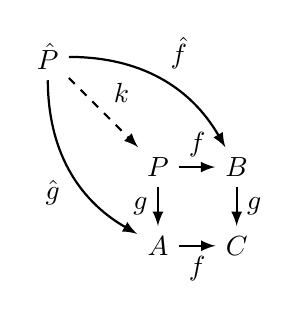
\begin{tikzpicture}[auto,>=latex, thick, scale=.5]
\node (P) {$P$};
\node (B) [right of=P] {$B$};
\node (A) [below of=P] {$A$};
\node (C) [below of=B] {$C$};
\node (P1) [node distance=1.4cm, left of=P, above of=P] {$\hat{P}$};
\draw[->] (P) to node {$f$} (B);
\draw[->] (P) to node [swap] {$g$} (A);
\draw[->] (A) to node [swap] {$f$} (C);
\draw[->] (B) to node {$g$} (C);
\draw[->, bend right] (P1) to node [swap] {$\hat{g}$} (A);
\draw[->, bend left] (P1) to node {$\hat{f}$} (B);
\draw[->, dashed] (P1) to node {$k$} (P);
\end{tikzpicture}


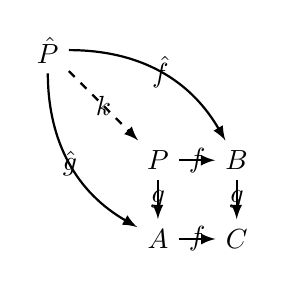
\begin{tikzpicture}[>=latex, thick, scale=2]
\node (P) {$P$};
\node (B) [right of=P] {$B$};
\node (A) [below of=P] {$A$};
\node (C) [below of=B] {$C$};
\node (P1) [node distance=1.4cm, left of=P, above of=P] {$\hat{P}$};
\draw[->] (P) to node {$f$} (B);
\draw[->] (P) to node [swap] {$g$} (A);
\draw[->] (A) to node [swap] {$f$} (C);
\draw[->] (B) to node {$g$} (C);
\draw[->, bend right] (P1) to node [swap] {$\hat{g}$} (A);
\draw[->, bend left] (P1) to node {$\hat{f}$} (B);
\draw[->, dashed] (P1) to node {$k$} (P);
\end{tikzpicture}


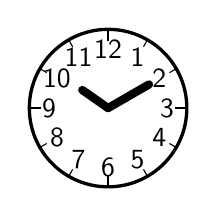
\begin{tikzpicture}[scale=.5]
\draw[very thick] (0,0) circle (2cm);%時計の外周
\foreach \angle / \label in 
  {0/3, 30/2, 60/1, 90/12, 120/11, 150/10, 180/9, 210/8, 240/7, 270/6, 300/5, 330/4} 
  { 
   \draw (\angle:1.8cm) -- (\angle:2cm); 
   \node at (\angle:1.5cm) {\textsf{\label}}; 
  } 
\foreach \angle in {0,90,180,270} 
   \draw[thick] (\angle:1.7cm) -- (\angle:2cm); 
\draw[line width=3pt, cap=round] (0,0) -- (145:0.8cm);%短針
\draw[line width=3pt, cap=round] (0,0) -- (30:1.2cm);%長針
\end{tikzpicture}%

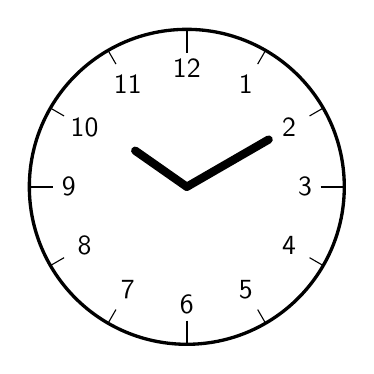
\begin{tikzpicture}
\draw[very thick] (0,0) circle (2cm);%時計の外周
\foreach \angle / \label in 
  {0/3, 30/2, 60/1, 90/12, 120/11, 150/10, 180/9, 210/8, 240/7, 270/6, 300/5, 330/4} 
  { 
   \draw (\angle:1.8cm) -- (\angle:2cm); 
   \node at (\angle:1.5cm) {\textsf{\label}}; 
  } 
\foreach \angle in {0,90,180,270} 
   \draw[thick] (\angle:1.7cm) -- (\angle:2cm); 
\draw[line width=3pt, cap=round] (0,0) -- (145:0.8cm);%短針
\draw[line width=3pt, cap=round] (0,0) -- (30:1.2cm);%長針
\end{tikzpicture}%

%%%%%%%%%%%%%%
\newpage
 \setcounter{page}{1}
 \addtocounter{footnote}{-4}
\begin{abstract}
切り分けのために、
pdf\_page\_splitter.shとファイル名変更のためのscript.awkを作成しました。
(というのはおおげさで、それぞれ数行程度のかんたんなものです。)


おおもとのpdfファイルができあがっているという前提です。

大まかな使いかたは以下のとおりです。
\end{abstract}

\section*{切り分け}


高校の情報が格納されているhighschool.pdf\footnote{おおもとのファイル名は半角英数字だけにしておくほうが無難です。}というファイルがあるとします。

このファイルは121ページあり、それぞれのページに各高校の情報が格納されています。

highschool.pdfがあるフォルダからコマンドプロンプトを開いて
\begin{screen}
\begin{verbatim}
pdf_page_splitter.sh highschool.pdf
\end{verbatim}
\end{screen}
とします。

これで、おおもとのpdfファイルから拡張子`.pdf'をとりのぞいたhighschoolというフォルダが自動的に作成されます。
そしてそのフォルダ中に各ページを切り分けた121個の
pdfファイルが自動的に作成されます。

各ファイルは、順番に
highschool\_001.pdf,
highschool\_002.pdf,
highschool\_003.pdf, \ldots
highschool\_121.pdf
となります。

命名規則は
\begin{quote}
`おおもとのファイル名'\_3桁の数字.pdf
\end{quote}
です\footnote{%
もともとのファイル名がkashiwa.pdfであれば、
kashiwaというフォルダにkashiwa\_001.pdf, kashiwa\_002.pdfみたいになるわけです。}。


\section*{ファイル名変更}
ファイル名に具体的な学校名をいれたいのであれば
\begin{screen}
\begin{verbatim}
hishschool_001,千葉
highschool_002,千葉女子
highschool_003,千葉東
highschool_004,千葉商業\hspace{10pt}以下省略
\end{verbatim}
\end{screen}
というファイルbase\_data.csvを作成します。

つぎに
\begin{screen}
\begin{verbatim}
awk -f script.awk base_data.csv | nkf -s > rename.sh
rename.sh
\end{verbatim}
\end{screen}
とすれば、ファイル名が学校名になったpdfがページ数の数だけできます。

具体的には、千葉.pdf, 千葉女子.pdf, 千葉東.pdf, 千葉商業.pdf\ldots{}みたいに121個のファイル名が書き換えられます。


なお、ファイル名を学校名にするのはいいとして、001千葉.pdfのように数字を振っておくほうがソートするときなど、後々の使い勝手はいいとおもう。その場合は先ほどのcsvファイルに数字をいれておけばいい。
ただし、どういう数字を使うかは要検討。


\section*{スクリプトの中身}

\begin{tcolorbox}[title=pdf\_page\_splitter.sh]
\begin{verbatim}
#!/bin/bash
for x in *.pdf; do
    output=${x%.pdf}
    mkdir -p "./${output}"
    pdfseparate "$x" "./${output}/${output}_%03d.pdf"
done
\end{verbatim}
\end{tcolorbox}

\begin{tcolorbox}[title=script.awk]
\begin{verbatim}
BEGIN {
    FS = ","
    print "#!/bin/bash"
}
{
    printf("mv ./%s.pdf ./%s.pdf \n", $1, $2)
}
\end{verbatim}
\end{tcolorbox}

\begin{tcolorbox}[title=rename.sh(これはscript.awkから自動的にできあがるもの)]
\begin{verbatim}
#!/bin/bash
mv ./highschool_001.pdf ./千葉.pdf 
mv ./highschool_002.pdf ./千葉女子q.pdf 
mv ./highschool_003.pdf ./千葉東.pdf 
mv ./highschool_004.pdf ./千葉商業.pdf \end{verbatim}
\end{tcolorbox}

\end{document}

